% This example is meant to be compiled with lualatex or xelatex
% The theme itself also supports pdflatex
\PassOptionsToPackage{unicode}{hyperref}
\documentclass[aspectratio=1610, 9pt]{beamer}

% Load packages you need here
\usepackage{polyglossia}
\setmainlanguage{english}

\usepackage{csquotes}
    

\usepackage{amsmath}
\usepackage{amssymb}
\usepackage{mathtools}

\usepackage{hyperref}
\usepackage{bookmark}
\usepackage{siunitx}

\usepackage[many]{tcolorbox}

\definecolor{light-gray}{gray}{0.95} %the shade of grey that stack exchange uses


\usepackage{fontspec}

\usepackage{transparent}

\usepackage{caption}
\captionsetup{justification=justified}

\usepackage[export]{adjustbox}

\usepackage{tikz}
\usetikzlibrary{shapes, arrows, backgrounds, fit, tikzmark, arrows.meta, calc, quotes, angles}

\newcommand{\credit}[1]{\par\hspace{0.5\textwidth} \tiny Credit:~\itshape#1}

% load the theme after all packages

\usetheme[
  showtotalframes, % show total number of frames in the footline
]{tudo}

% Put settings here, like
\unimathsetup{
  math-style=ISO,
  bold-style=ISO,
  nabla=upright,
  partial=upright,
  mathrm=sym,
}

\setlength{\footerleftwidth}{0.3\textwidth}
\setlength{\footercenterwidth}{0.4\textwidth}
\setlength{\footerrightwidth}{0.3\textwidth}

\title{High-energy lepton and photon simulations with the framework PROPOSAL}
\author[jean-marco.alameddine@tu-dortmund.de]{Jean-Marco Alameddine, Pascal Gutjahr}
\institute[]{Astroparticle Physics WG Rhode - TU Dortmund University}
\titlegraphic{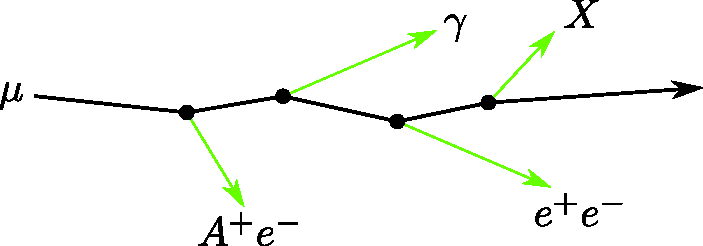
\includegraphics[width=0.7\textwidth]{images/muon_path.pdf}}
\date[]{}


\begin{document}

\setbeamertemplate{caption}{\raggedright\insertcaption\par}

\maketitle

\section{Introduction}

\begin{frame}[plain,c,noframenumbering]
  \begin{center}
    \Huge Introduction to PROPOSAL
  \end{center}
\end{frame}

\begin{frame}
  \centering
  \Huge
  \textbf{Motivation behind PROPOSAL}\\
  \large
  (and many other Monte Carlo Simulation tools...)
  \vspace{5mm}
  \begin{columns}[t]
        \begin{column}{0.45\textwidth}
            \centering
            \textbf{Theory:}
          \begin{minipage}[c]{\textwidth}
            \centering
            \vspace{2mm}
                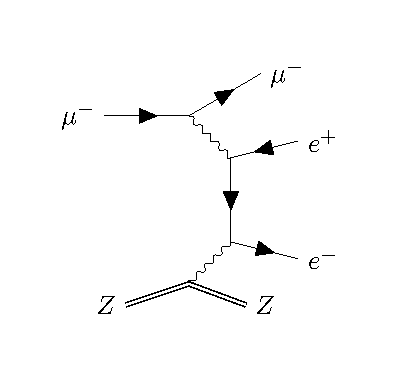
\includegraphics[trim=25 25 30 30, clip, width=0.6\textwidth]{images/feynman/epair_feynman.pdf}
        \end{minipage}%
        \end{column}
        \begin{column}{0.05\textwidth}
          \vspace{12mm}\\
          \Huge\textbf{\rightarrow}
        \end{column}
        \begin{column}{0.45\textwidth}
          \centering
            \textbf{Event signatures:}
            \begin{minipage}[c]{\textwidth}
              \vspace{4mm}
            \centering
                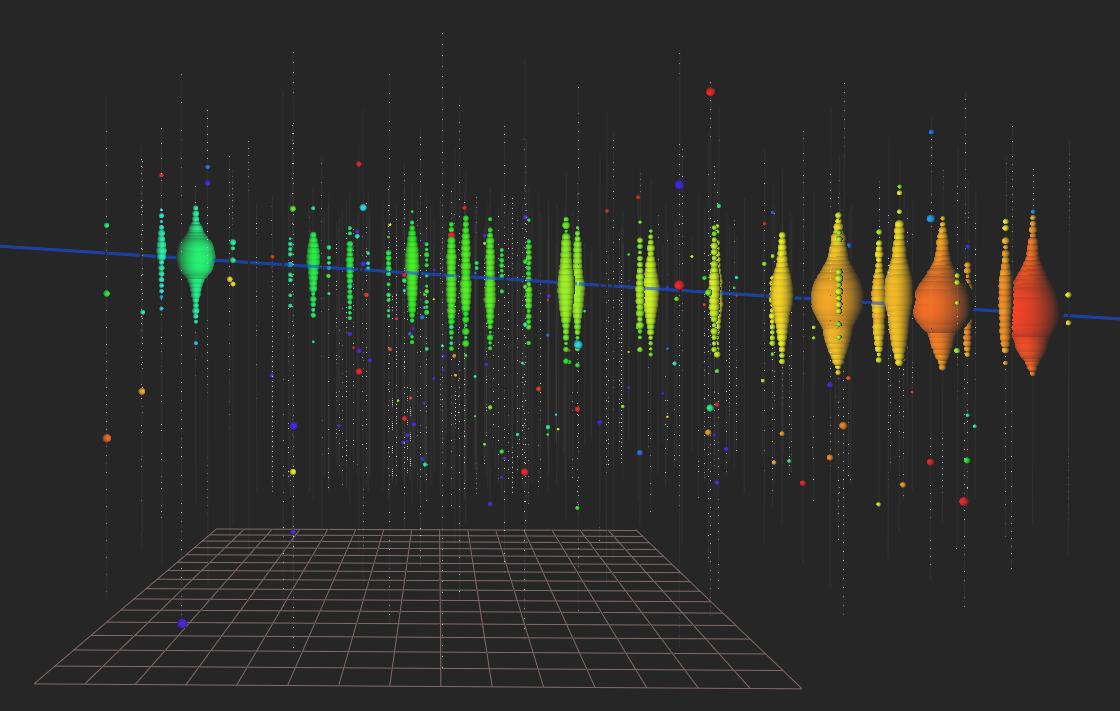
\includegraphics[width=0.8\textwidth]{images/Track.png}
                \credit{IceCube Collaboration}
        \end{minipage}%
        \end{column}
    \end{columns}
\end{frame}


\begin{frame}{}
  \vspace{-3cm}
  \begin{minipage}[t][1cm][t]{\textwidth}
  {\huge \textbf{PROPOSAL}} {\huge\textbf{\rightarrow}}
  \pgfsetfillopacity{0}\colorbox{tugreen}{\pgfsetfillopacity{1}{\huge \textbf{P}}{\Large ropagator}}{\Large with}\pgfsetfillopacity{0}\colorbox{tugreen}{\pgfsetfillopacity{1}{\huge \textbf{O}}{\Large ptimal }{\huge \textbf{P}}{\Large recision and }{\huge \textbf{O}}{\Large ptimized }{\huge \textbf{S}}{\Large peed}}{\Large for}\pgfsetfillopacity{0}\colorbox{tugreen}{\pgfsetfillopacity{1}{\huge \textbf{A}}ll {\huge \textbf{L}}{\Large eptons}}
  \end{minipage}
  \begin{minipage}[t][1cm][t]{\textwidth}
    
  \end{minipage}
\end{frame}

\begin{frame}{}
  \vspace{-3cm}
  \begin{minipage}[t][1cm][t]{\textwidth}
  {\huge \textbf{PROPOSAL}} {\huge\textbf{\rightarrow}}
  \pgfsetfillopacity{0.9}\colorbox{tugreen}{\pgfsetfillopacity{1}{\huge \textbf{P}}{\Large ropagator}}{\Large with}\pgfsetfillopacity{0}\colorbox{tugreen}{\pgfsetfillopacity{1}{\huge \textbf{O}}{\Large ptimal }{\huge \textbf{P}}{\Large recision and }{\huge \textbf{O}}{\Large ptimized }{\huge \textbf{S}}{\Large peed}}{\Large for}\pgfsetfillopacity{0}\colorbox{tugreen}{\pgfsetfillopacity{1}{\huge \textbf{A}}ll {\huge \textbf{L}}{\Large eptons}}
  \end{minipage}
  \begin{minipage}[t][1cm][t]{\textwidth}
  \vspace{-5mm}
    \begin{columns}[onlytextwidth]
        \begin{column}{0.5\textwidth}
            \begin{itemize}
              \item 3D Monte Carlo simulation of individual particles, considering \ldots
              \begin{itemize}
                \item[\normalcolor{\ldots}] energy losses
                \item[\normalcolor{\ldots}] scattering effects
                \item[\normalcolor{\ldots}] particle decays
                \item[$\rightarrow$] \textbf{Customizable:} Selection of different parametrizations available for each process
              \end{itemize}
              \item \textbf{Input:} Initial particle state
              \item \textbf{Output:} Information on particle track, including \ldots
              \begin{itemize}
                \item[\normalcolor{\ldots}] Final particle state
                \item[\normalcolor{\ldots}] Energy losses
                \item[\normalcolor{\ldots}] Intermediate particle states
              \end{itemize}
              \item C\texttt{++}14/Python library
            \end{itemize}
        \end{column}
        \begin{column}{0.5\textwidth}
            \begin{figure}
                \centering
                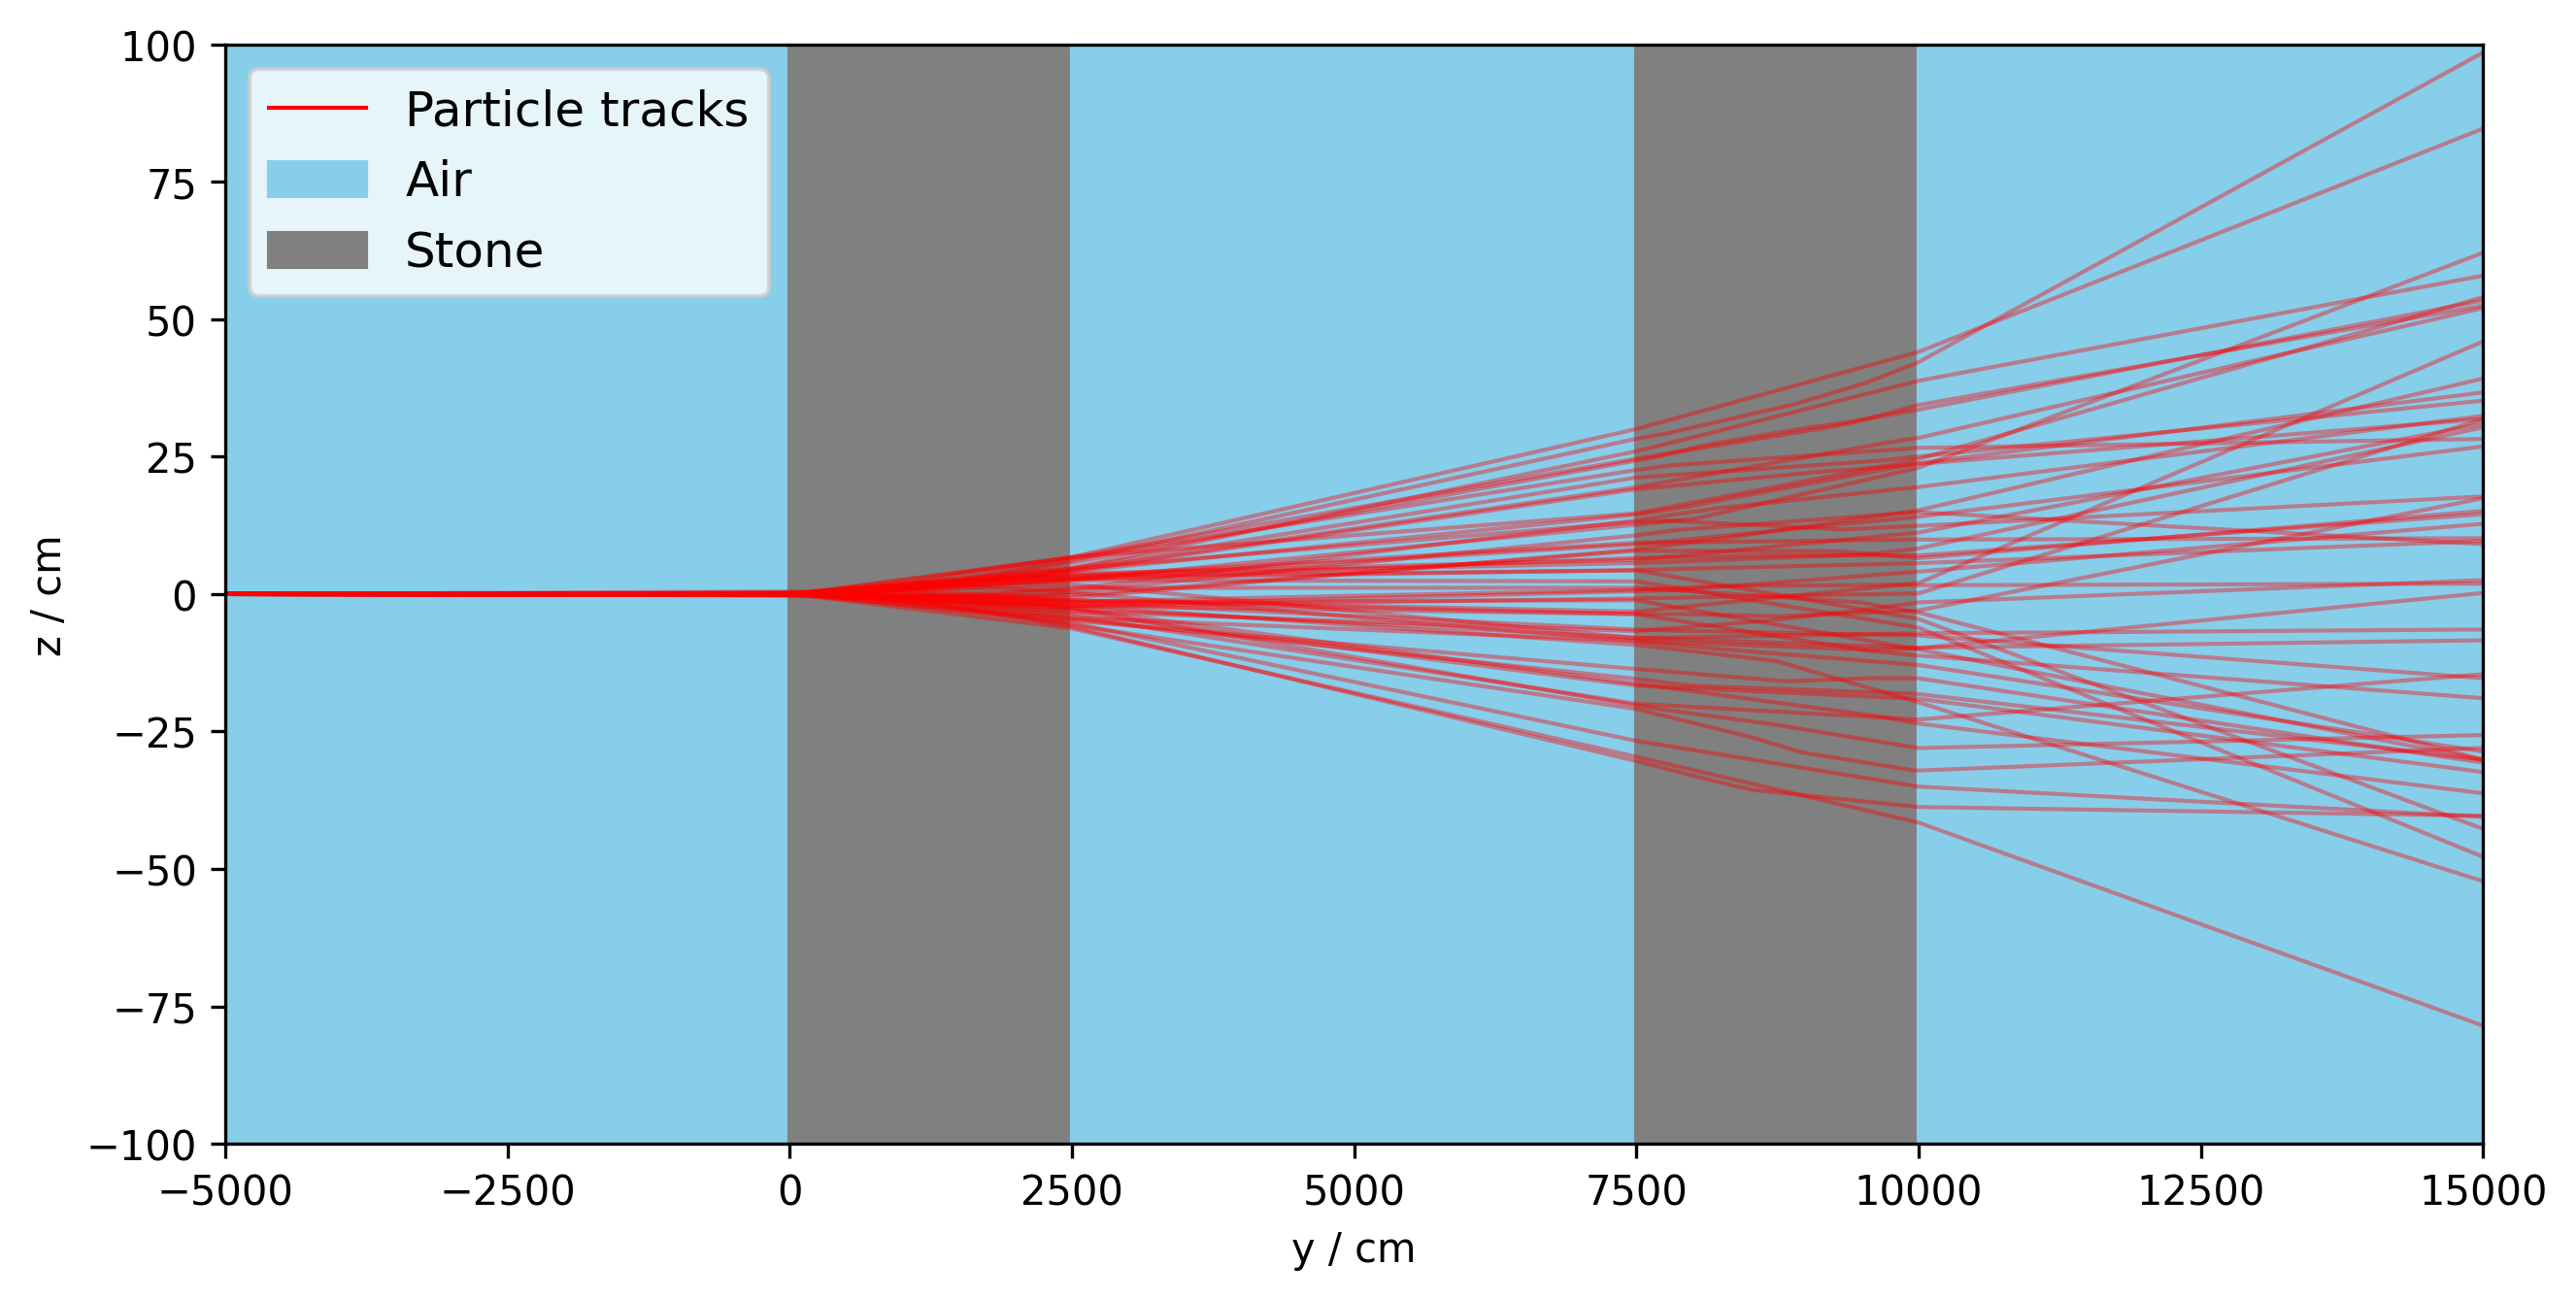
\includegraphics[width=0.85\textwidth]{plots/tracks.png}
            \end{figure}
            \vspace{-3mm}
            \begin{figure}
                \centering
                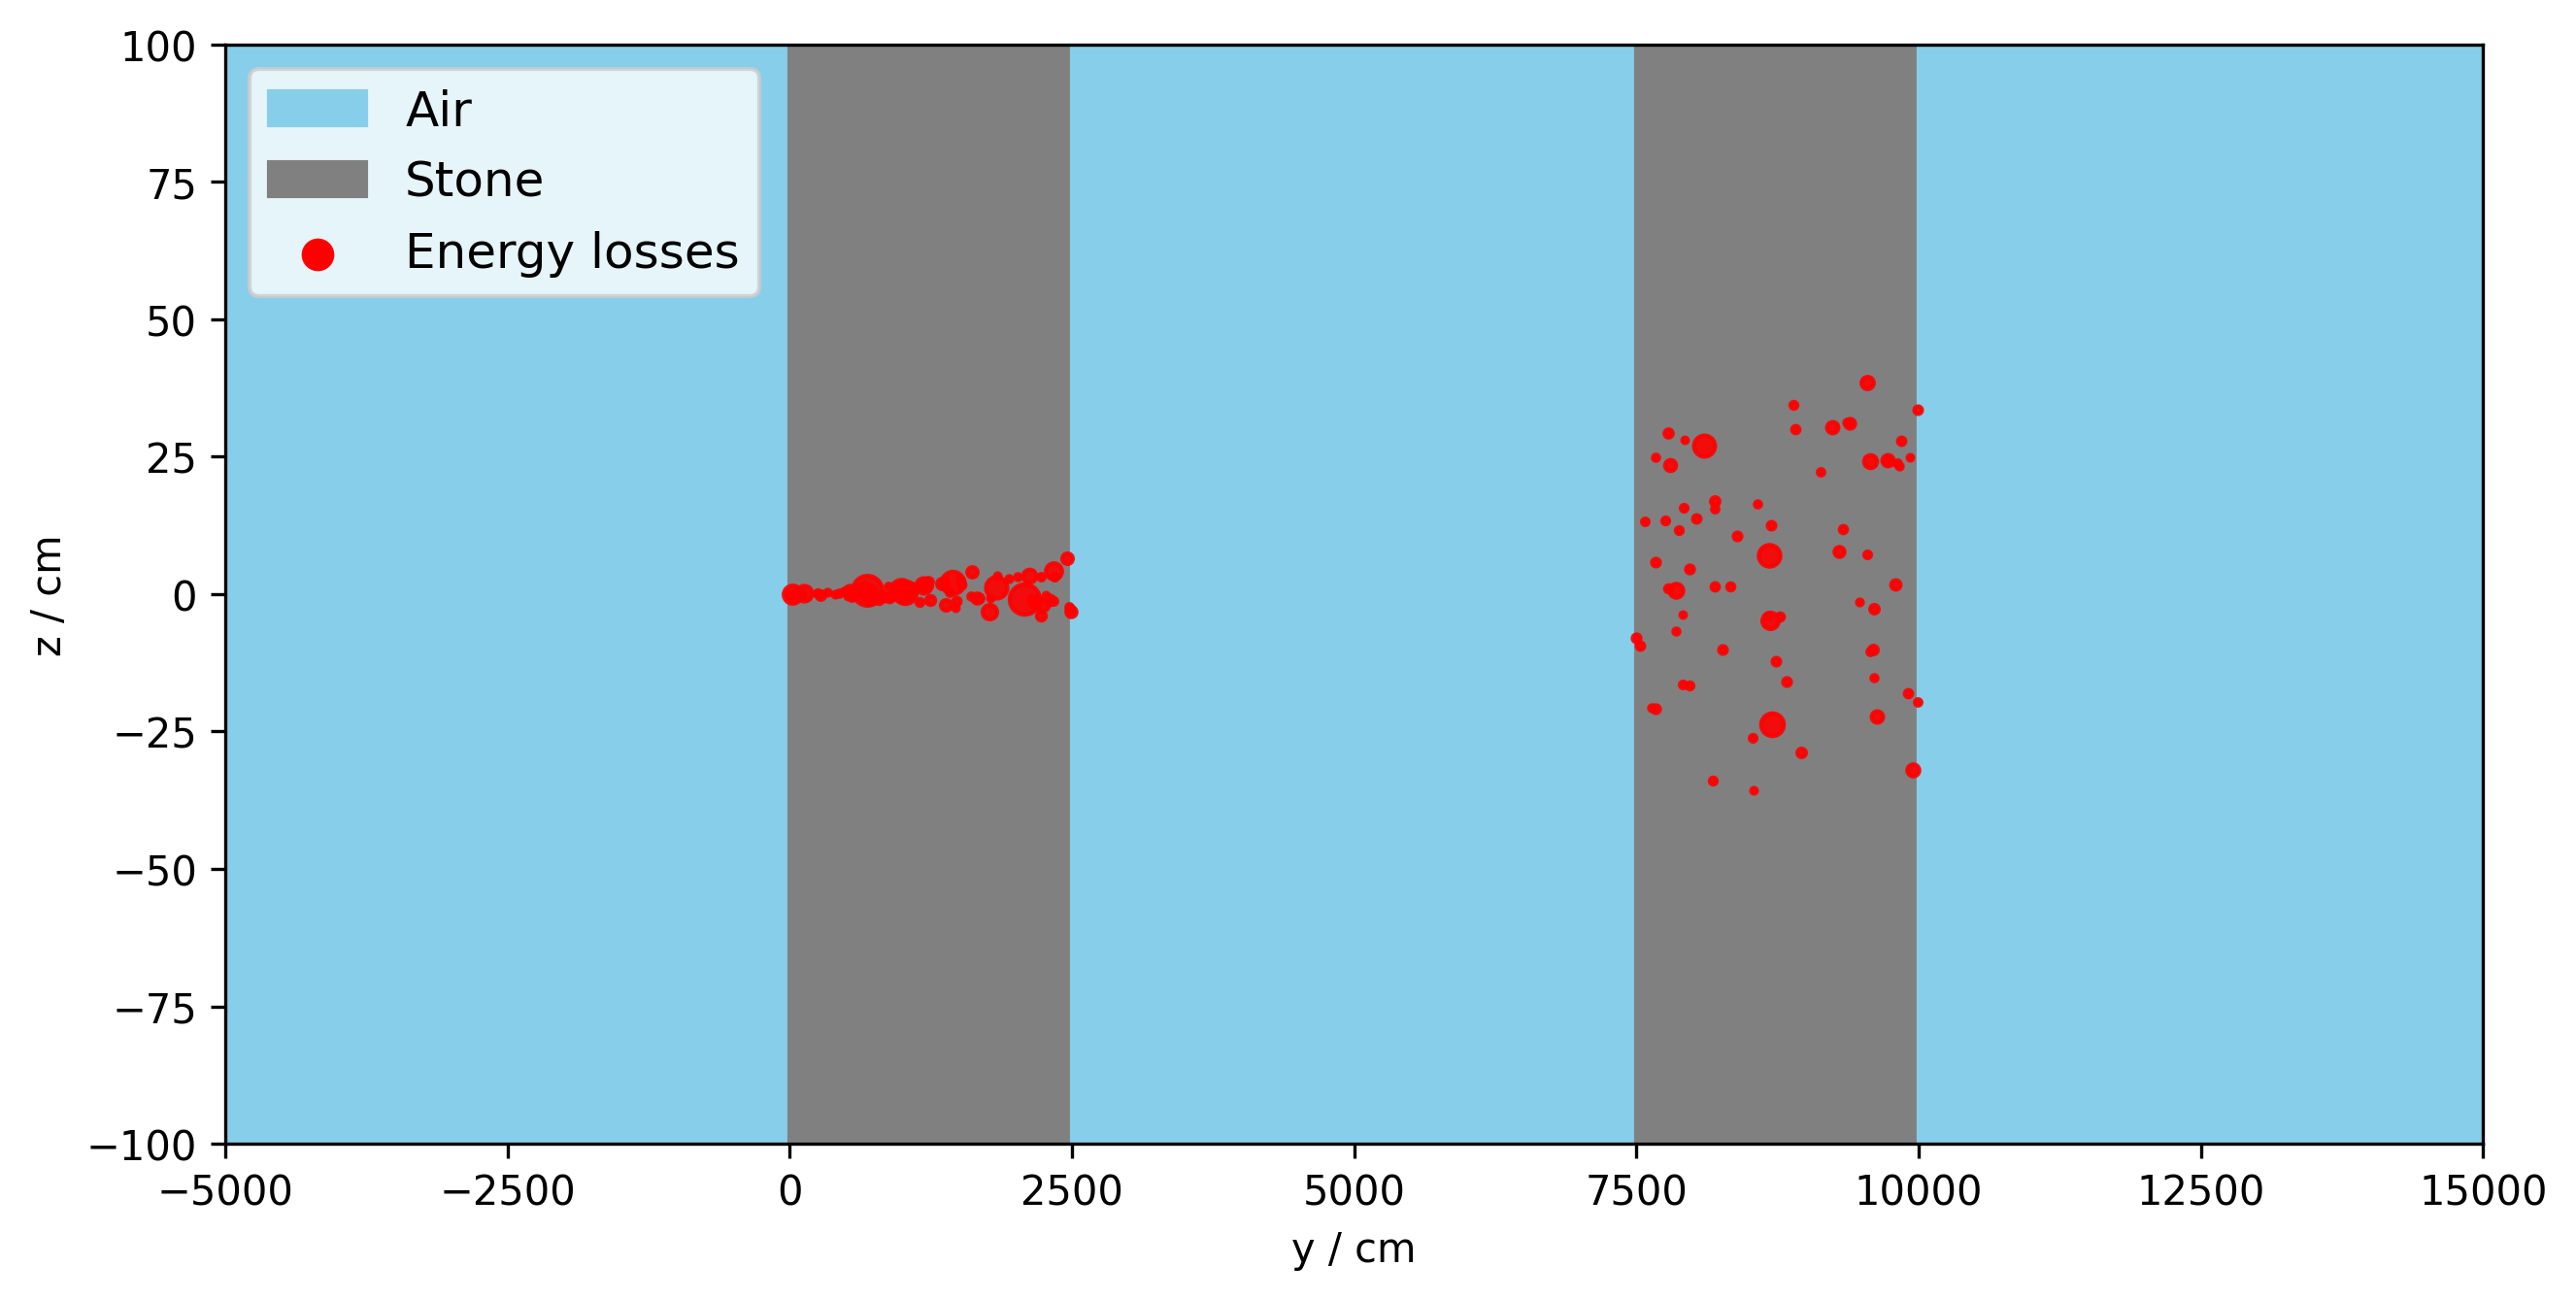
\includegraphics[width=0.85\textwidth]{plots/losses.png}
            \end{figure}
        \end{column}
    \end{columns}

  \end{minipage}
\end{frame}


\begin{frame}{}
  \vspace{-3cm}
  \begin{minipage}[t][1cm][t]{\textwidth}
  {\huge \textbf{PROPOSAL}} {\huge\textbf{\rightarrow}}
  \pgfsetfillopacity{0}\colorbox{tugreen}{\pgfsetfillopacity{1}{\huge \textbf{P}}{\Large ropagator}}{\Large with}\pgfsetfillopacity{0.9}\colorbox{tugreen}{\pgfsetfillopacity{1}{\huge \textbf{O}}{\Large ptimal }{\huge \textbf{P}}{\Large recision and }{\huge \textbf{O}}{\Large ptimized }{\huge \textbf{S}}{\Large peed}}{\Large for}\pgfsetfillopacity{0}\colorbox{tugreen}{\pgfsetfillopacity{1}{\huge \textbf{A}}ll {\huge \textbf{L}}{\Large eptons}}
  \end{minipage}
  \begin{minipage}[t][1cm][t]{\textwidth}
    \begin{columns}[onlytextwidth]
        \begin{column}{0.5\textwidth}
          \textbf{Interpolation tables:}
            \begin{itemize}
              \item Cross sections and results of propagation integrals are stored as interpolation tables
              \begin{itemize}
                %\item[$\rightarrow$] We use the \href{https://github.com/tudo-astroparticlephysics/cubic_interpolation}{CubicInterpolation} library 
                \item[$\rightarrow$] Crucial for the performance of PROPOSAL
              \end{itemize}
            \end{itemize}
          \textbf{Energy loss cuts:}
          \begin{itemize}
            \item PROPOSAL differentiates between continuous and stochastic energy losses
            \item Energy losses can be defined by their relative size $v_\text{loss}$ and their absolute size $e_\text{loss}$
            \item The energy cut settings ($v_\text{cut}, e_\text{cut}$) define which interactions are treated stochastically/continuously
            %\begin{itemize}
            %  \item[$\rightarrow$] Adjust energy cut settings to find ideal trade-off between precision and performance
            %\end{itemize}
          \end{itemize}
        \end{column}
        \begin{column}{0.5\textwidth}

          \begin{figure}
            \tikzstyle{vspecies_blue}=[rectangle, minimum size=0.5cm,draw=black,fill=cyan, fill opacity=1.0, text opacity=1]
            \tikzstyle{vspecies_red}=[rectangle, minimum size=0.5cm,draw=black,fill=red, fill opacity=1.0, text opacity=1]

            \begin{tikzpicture}[>=latex,shorten >=2pt,shorten <=2pt,shape aspect=1]


            \coordinate (A) at (0, 0);

            \draw[draw=none, fill=cyan, fill opacity=1.0] ($ (A) + (-3,-2) $) rectangle ++(6, 4);

            \draw[draw=none,fill=red, fill opacity=1.0] ($ (A) + (0, 0.07) $) circle (7.0ex);

            \node [cylinder, shape border rotate=90, draw,minimum height=1cm,minimum width=0.75cm] (c) at (A) {};

            \node [vspecies_blue] (a) at (-1.1, 2.5) {\small{$v_\text{cut} = \num{0.05}$}} ;
            \node [vspecies_red] (b) at (1.1, 2.5) {\small{$e_\text{cut} = \SI{500}{\mega\electronvolt}$}} ;

            \draw [->, densely dotted, line width=0.4mm] ($0.33*(-3, 0.7)$) -- ($-0.05*(-3, 0.7)$) node [midway, above, sloped] (TextNode) {};

            \draw [loosely dotted, line width=0.4mm] ($0.95*(-3, 0.7)$) -- ($0.30*(-3, 0.7)$) node [near end, above, sloped] (TextNode) {$\mu$};

            \end{tikzpicture}
            \captionsetup{justification=centering}
            \caption*{$\rightarrow$ Adjust energy cut settings to find ideal \\trade-off between precision and performance!}
          \end{figure}

        \end{column}
    \end{columns}
  \end{minipage}
\end{frame}

\begin{frame}{}
  \vspace{-3cm}
  \begin{minipage}[t][1cm][t]{\textwidth}
  {\huge \textbf{PROPOSAL}} {\huge\textbf{\rightarrow}}
  \pgfsetfillopacity{0}\colorbox{tugreen}{\pgfsetfillopacity{1}{\huge \textbf{P}}{\Large ropagator}}{\Large with}\pgfsetfillopacity{0}\colorbox{tugreen}{\pgfsetfillopacity{1}{\huge \textbf{O}}{\Large ptimal }{\huge \textbf{P}}{\Large recision and }{\huge \textbf{O}}{\Large ptimized }{\huge \textbf{S}}{\Large peed}}{\Large for}\pgfsetfillopacity{0.9}\colorbox{tugreen}{\pgfsetfillopacity{1}{\huge \textbf{A}}ll {\huge \textbf{L}}{\Large eptons}}$\tikzmark{add}$


  \end{minipage}
  \begin{minipage}[t][1cm][t]{\textwidth}

  \vspace{-10pt}
  \begin{columns}[t]
    \column{.5\textwidth}
    \begin{figure}
      %\caption*{Muon energy losses:}
      %\vspace{-9pt}
      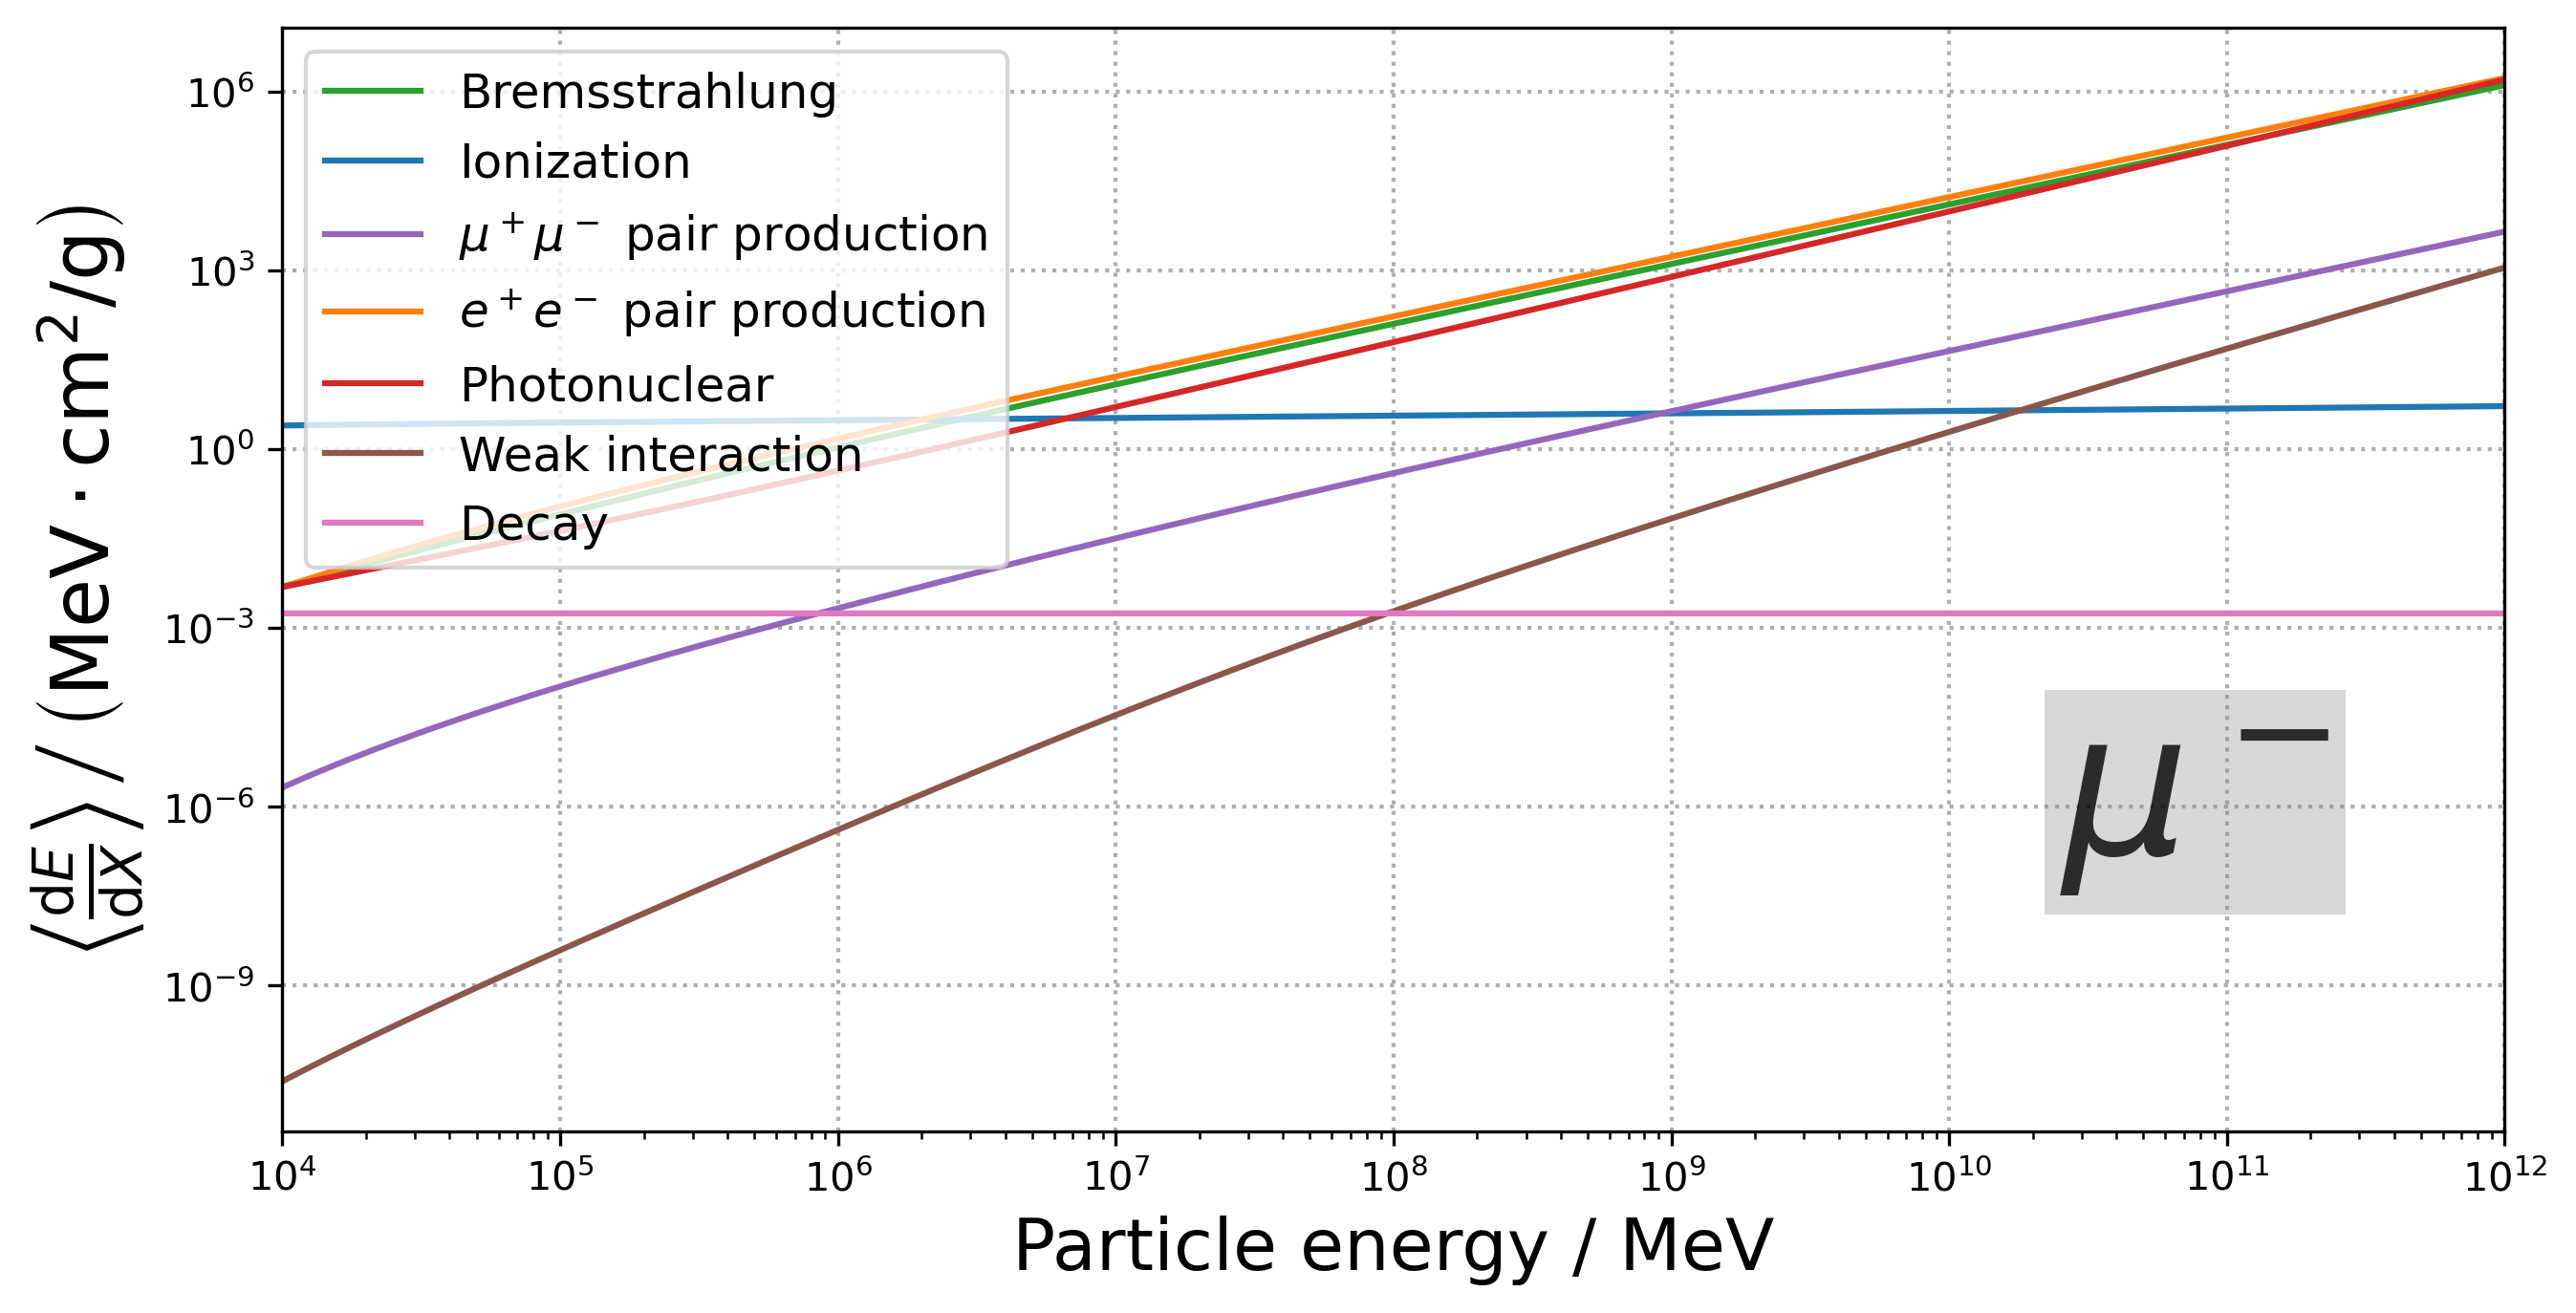
\includegraphics[width=\linewidth, height=.4\textheight, keepaspectratio]{plots/muon_dEdx.png}
    \end{figure}
    \vspace{-10pt}
    \begin{figure}
      %\caption*{Positron/Electron energy losses:}
      %\vspace{-9pt}
      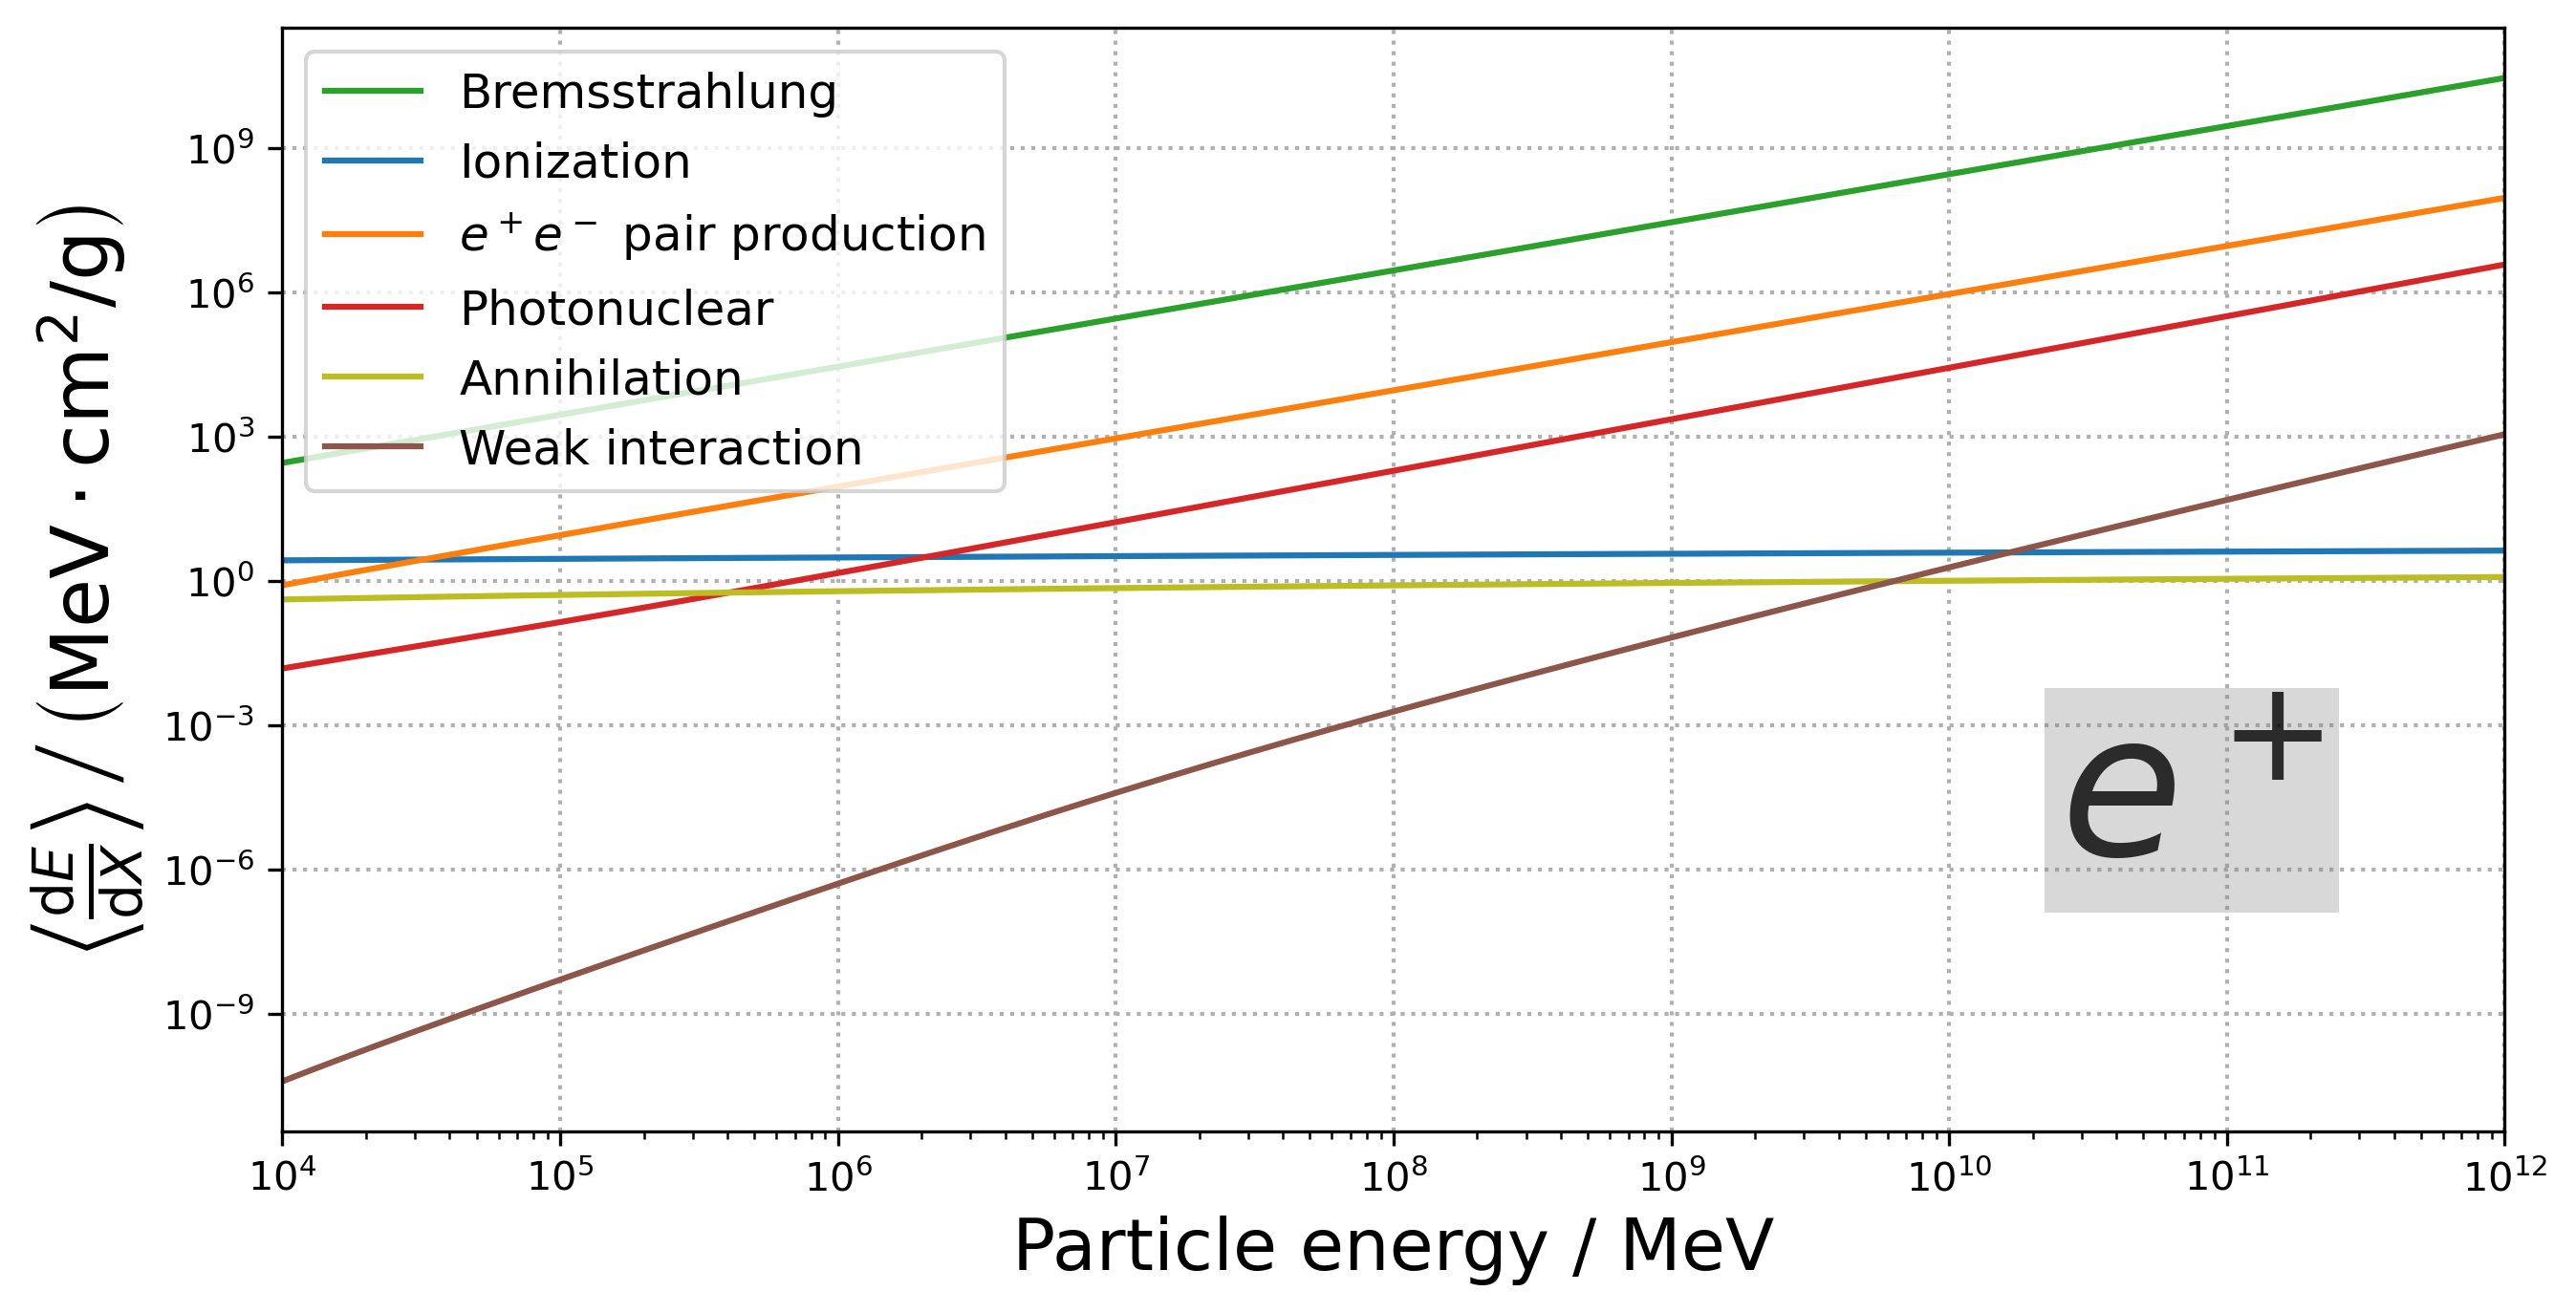
\includegraphics[width=\linewidth, height=.4\textheight, keepaspectratio]{plots/positron_dEdx.png}
    \end{figure}
    \vspace{-10pt}
    \column{.5\textwidth}
    \begin{figure}
      %\caption*{Tau energy losses:}
      %\vspace{-9pt}
      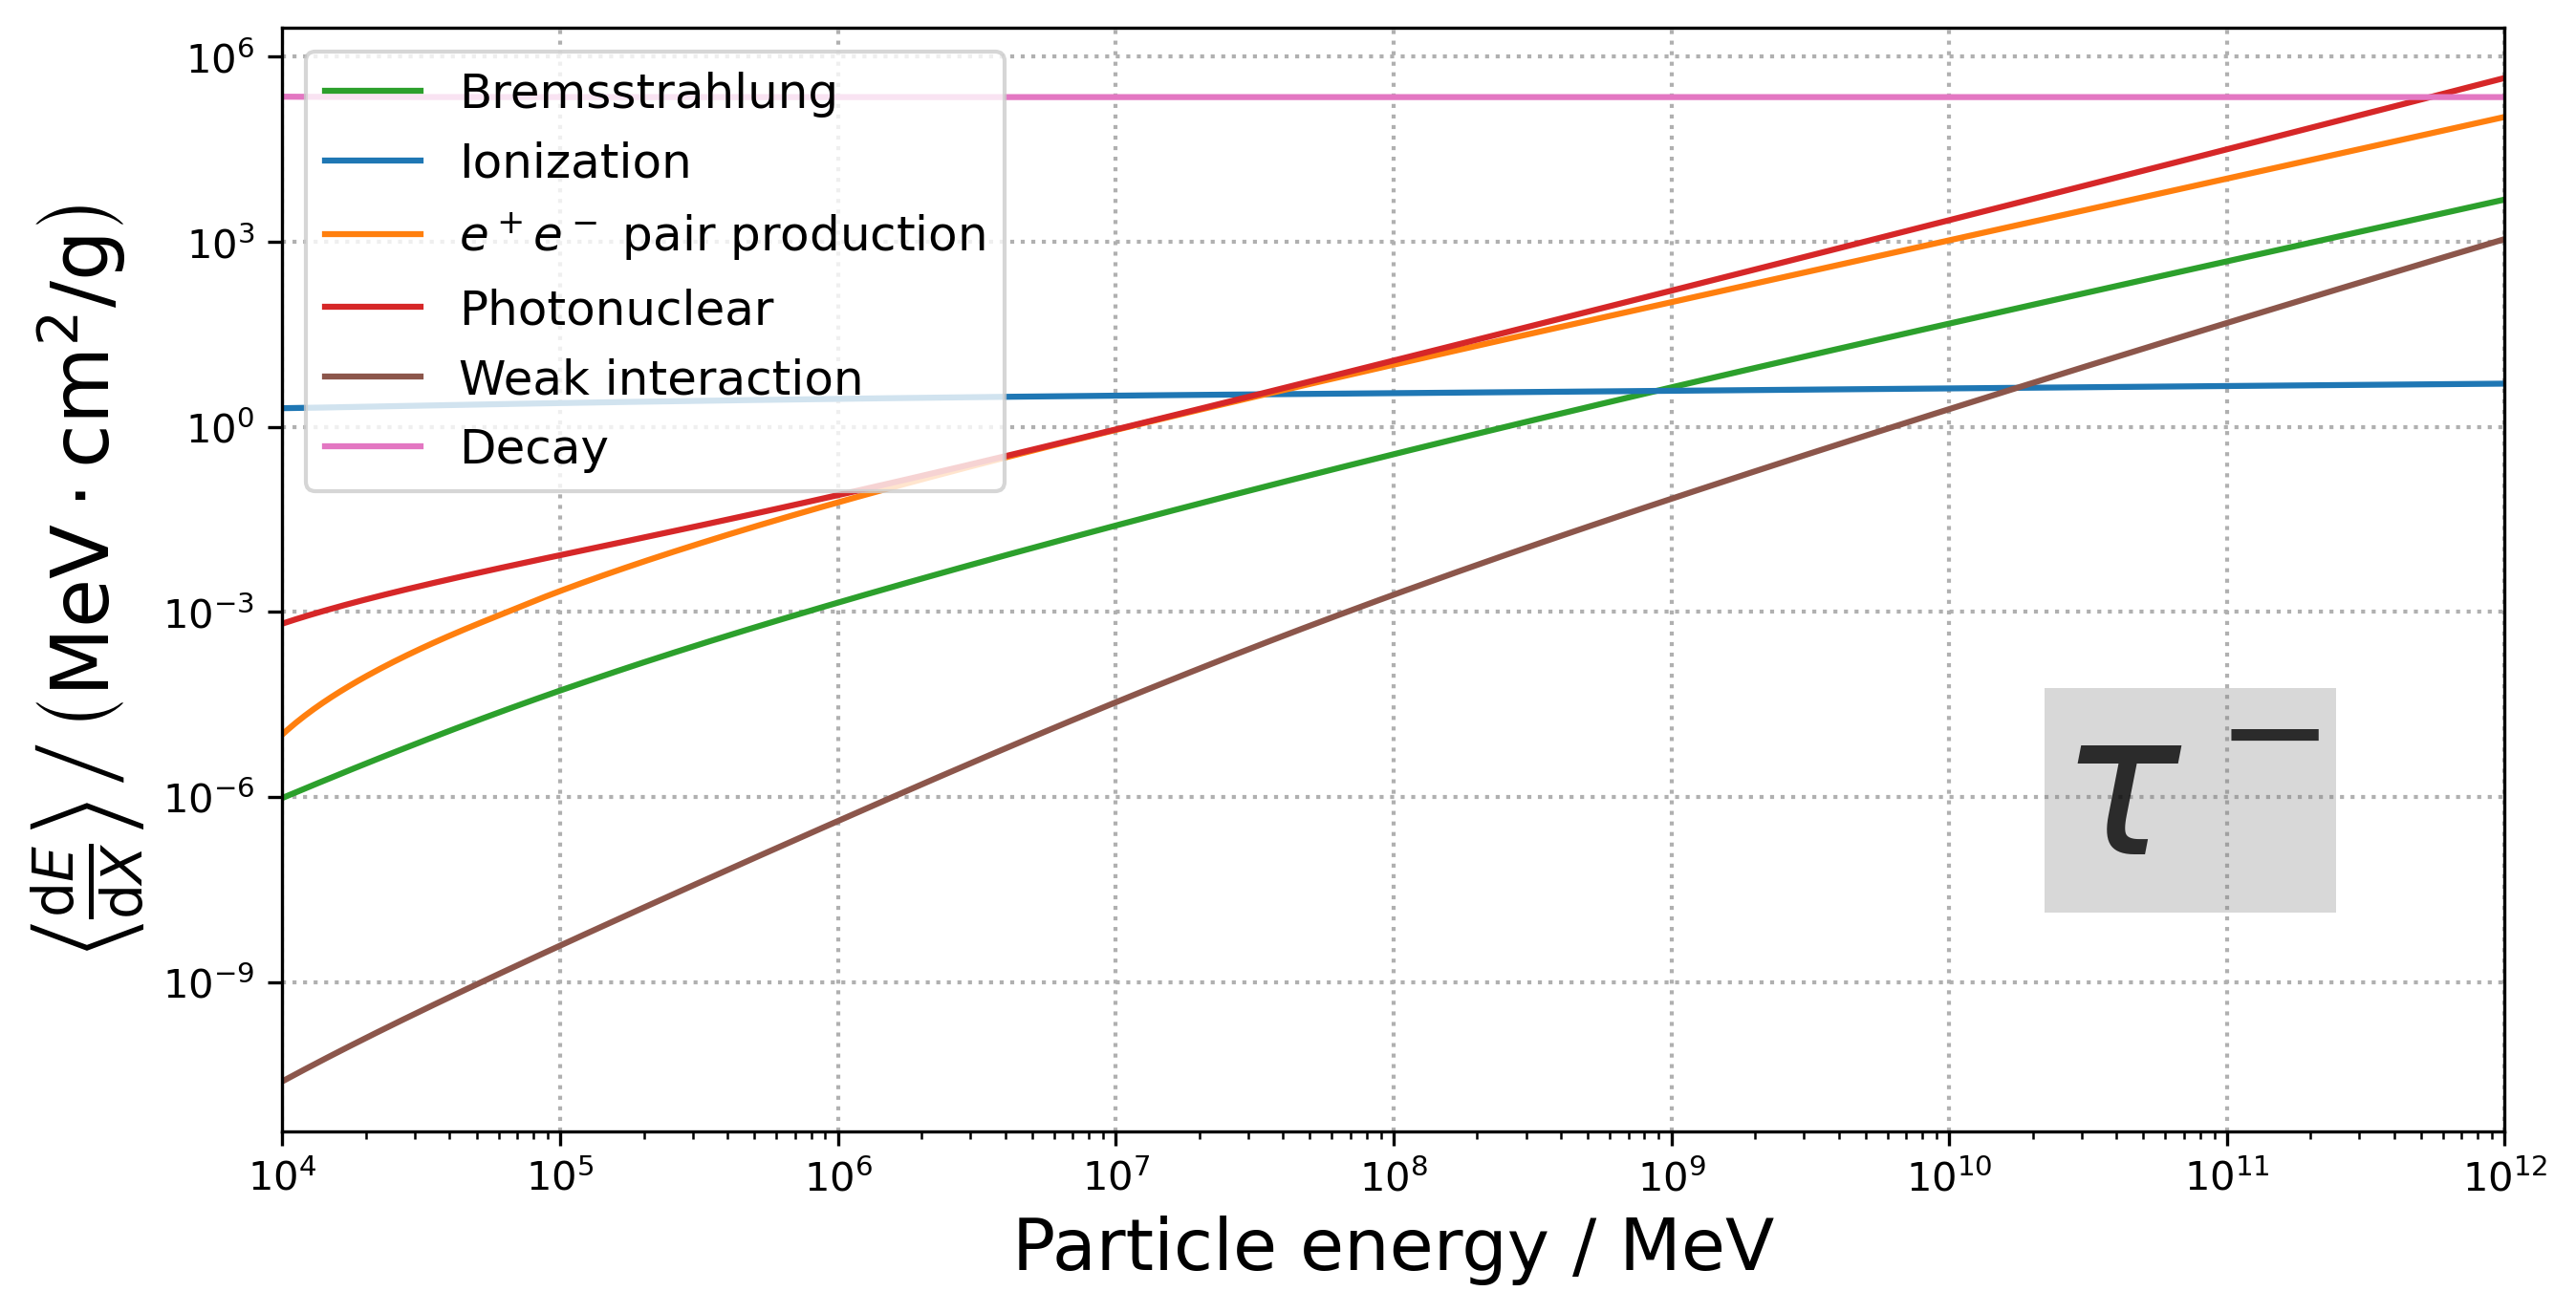
\includegraphics[width=\linewidth, height=.4\textheight, keepaspectratio]{plots/tau_dEdx.png}
    \end{figure}
    \vspace{-10pt}
    \begin{figure}
      %\caption*{High-energy photon energy losses:}
      %\vspace{-9pt}
      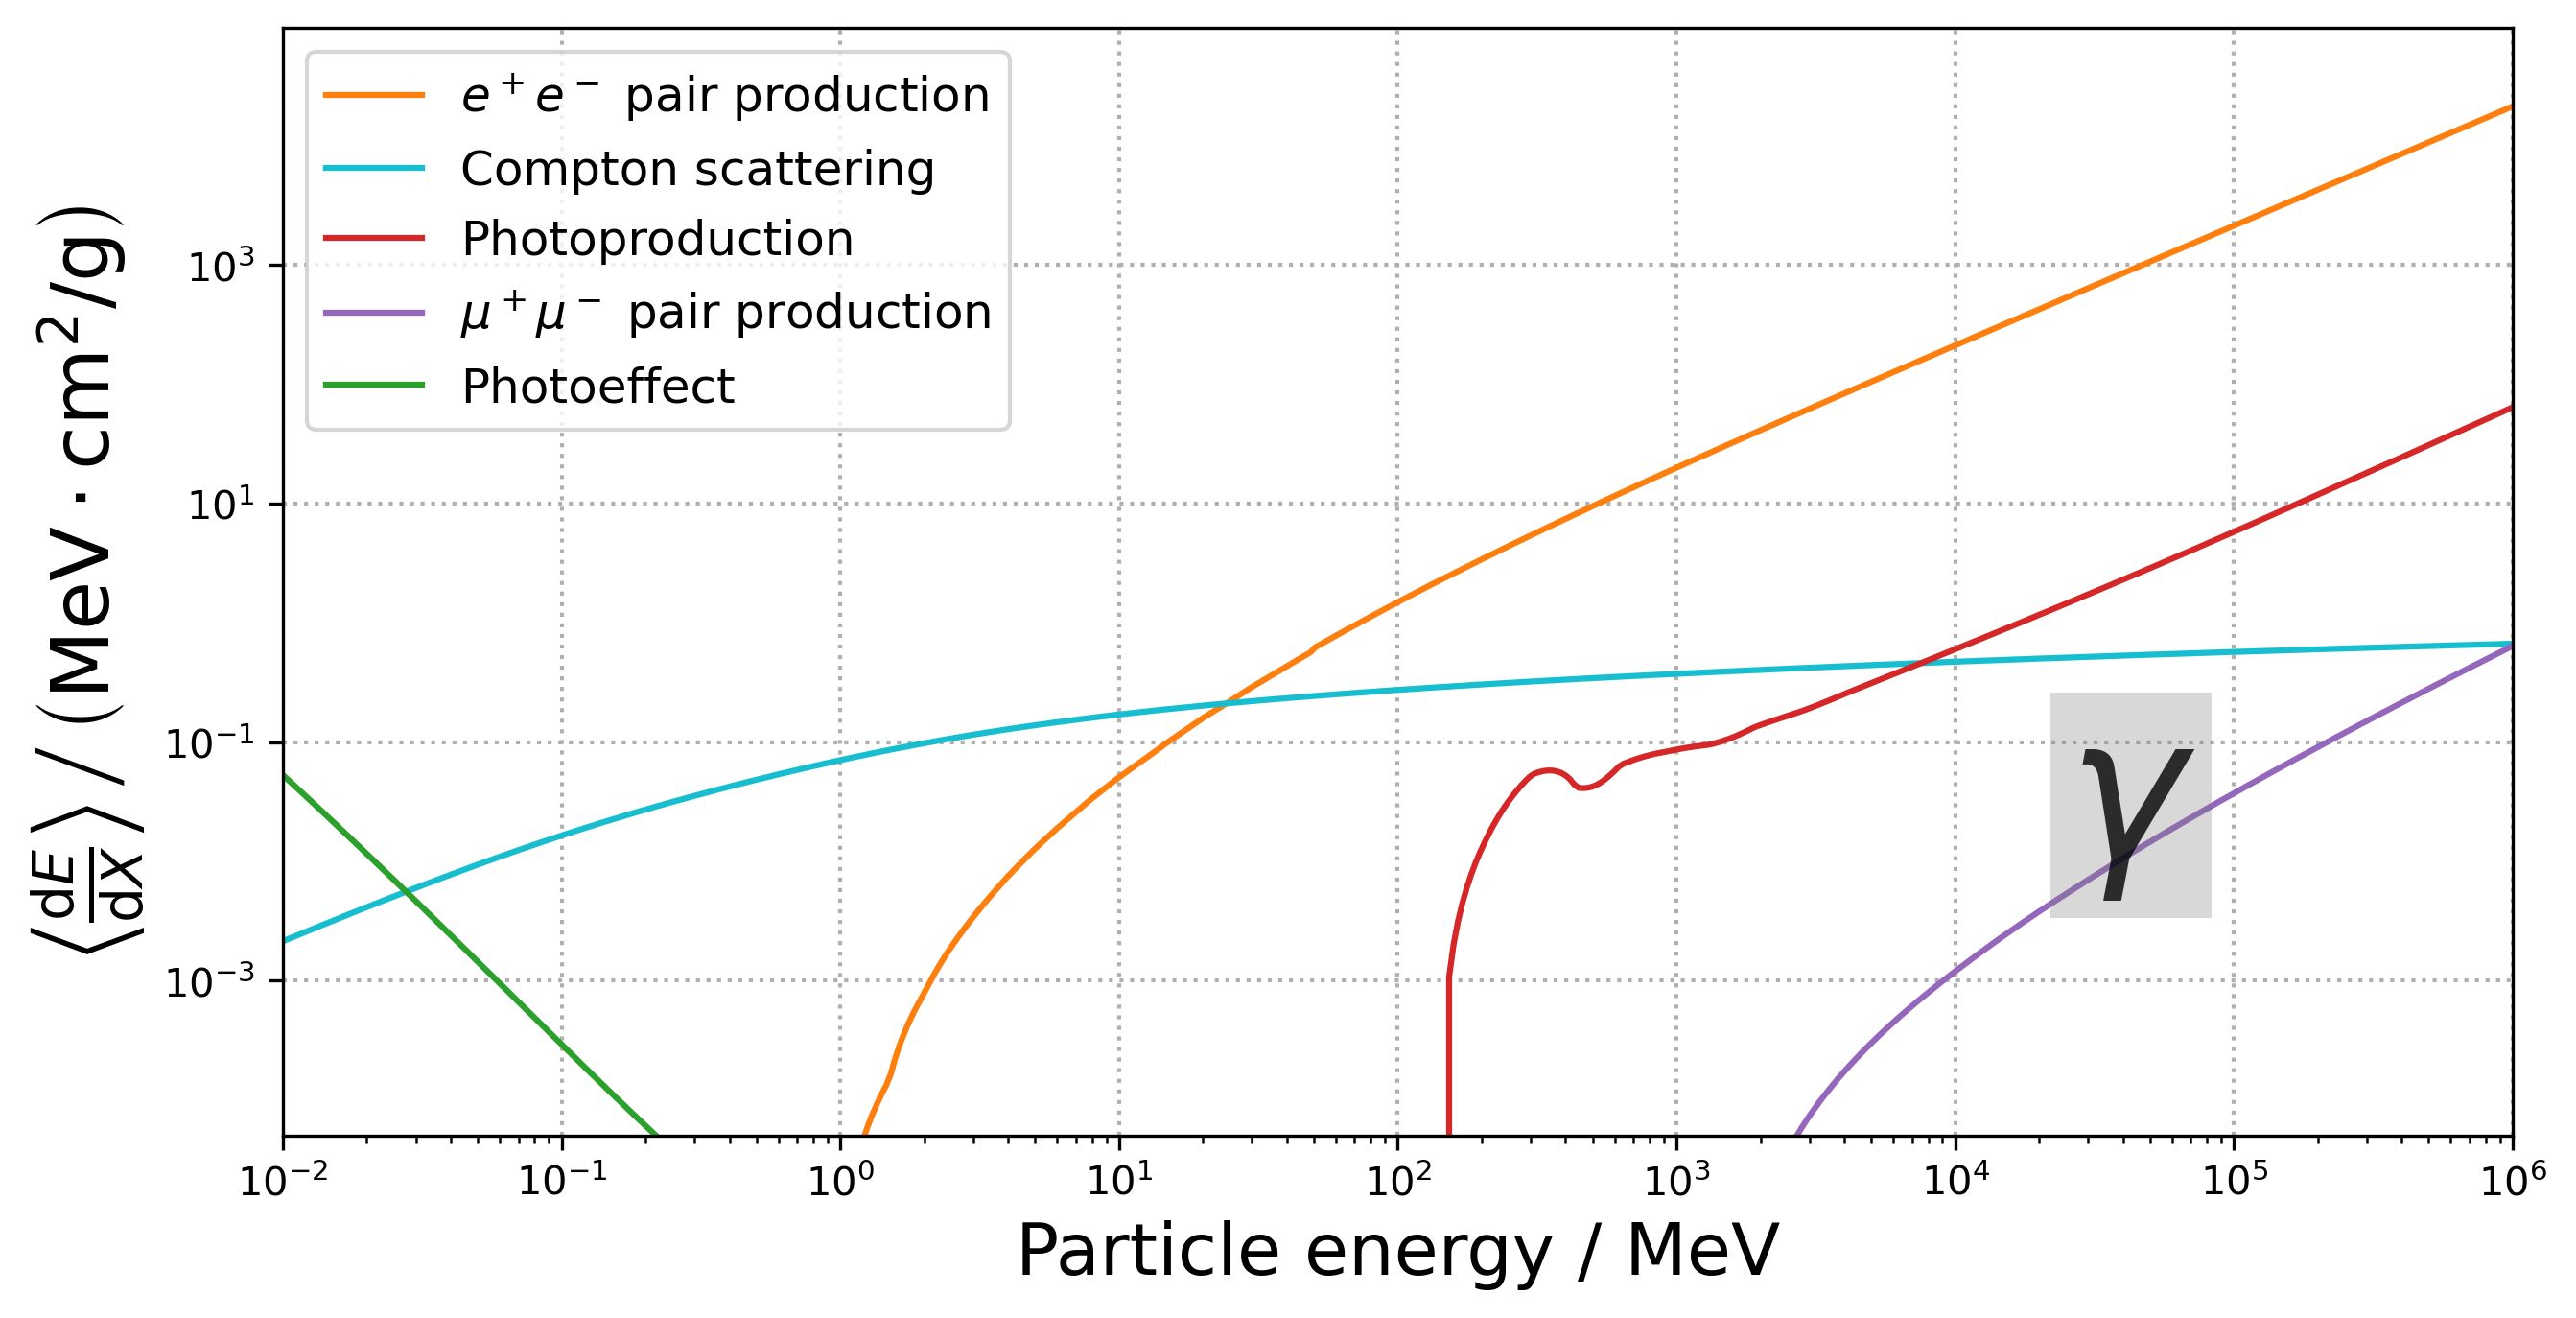
\includegraphics[width=\linewidth, height=.4\textheight, keepaspectratio]{plots/photon_dEdx.png}
    \end{figure}
  \end{columns}

  \end{minipage}
  \newfontfamily{\Chalkduster}{Chalkduster}

  \begin{tikzpicture}[overlay,remember picture]
    \node[text=red, rotate=10] (A) at ($({pic cs:add})+(-0.5ex,-2.7ex)$) {\Chalkduster and photons};
  \end{tikzpicture}

\end{frame}

% Maybe remove this slide and distribute it to the "Propagator" (C++/Python) and outlook slide (how to install)

\begin{frame}<presentation:0>[c]
  \begin{columns}[onlytextwidth]
  \begin{column}{0.6\textwidth}
  \textbf{Some technical details:}
  \begin{itemize}
      \setlength{\itemsep}{3pt}
      \item PROPOSAL is written in C\texttt{++}14, but callable from Python as well
          \begin{itemize}
              \item[\rightarrow] Easy python installation - Try: \texttt{pip install proposal}
              \item[\rightarrow] Easy usage in C\texttt{++} via the package manager \href{https://conan.io/center/proposal}{conan}
          \end{itemize}
      \item PROPOSAL is written in a modular and extentable way
          \begin{itemize}
              \item[\rightarrow] Selection of different parametrizations available for each physical process
              \item[\rightarrow] New parametrizations or processes can be added to PROPOSAL
          \end{itemize} 
      \item Actively maintained and developed as an open-source project
          \begin{itemize}
              \item[\rightarrow] Visit us on GitHub: \url{github.com/tudo-astroparticlephysics/PROPOSAL}
          \end{itemize}
  \end{itemize}
  \end{column}
  \begin{column}{0.4\textwidth}
    \begin{figure}
        \centering
        
\includegraphics[width=0.7\textwidth]{logos/cpp-python.png}
    \end{figure}
  \end{column}
  \end{columns}
\end{frame}

\section{Updates}

\begin{frame}[plain,c,noframenumbering]
  \begin{center}
    \Huge Recent updates in PROPOSAL
  \end{center}
\end{frame}

\begin{frame}

\begin{columns}[onlytextwidth]
    \begin{column}{0.45\textwidth}
    	\textbf{Improvements for electromagnetic interactions:}
    	\begin{itemize}
    		\item Inclusion of $\gamma \to \text{Hadrons}$ \\(Photohadronic interaction)
            \begin{itemize}
                \item[$\rightarrow$] Relevant for very-high energies
            \end{itemize}
    		%\item Sampling of deflection angles for bremsstrahlung photons
    		\item Inclusion of the photoeffect
            \begin{itemize}
                \item[$\rightarrow$] Relevant for low energies
            \end{itemize}
            \item Inclusion of $\gamma \to \mu^+ \mu^-$
            \begin{itemize}
                \item[$\rightarrow$] Relevant signatures (source of $\mu$-pairs in electromagnetic showers)
            \end{itemize}
    	\end{itemize}

    	%\hspace{10pt} $\Rightarrow$ More about this later!

    \end{column}
    \begin{column}{0.55\textwidth}

    \begin{figure}
    	\centering
        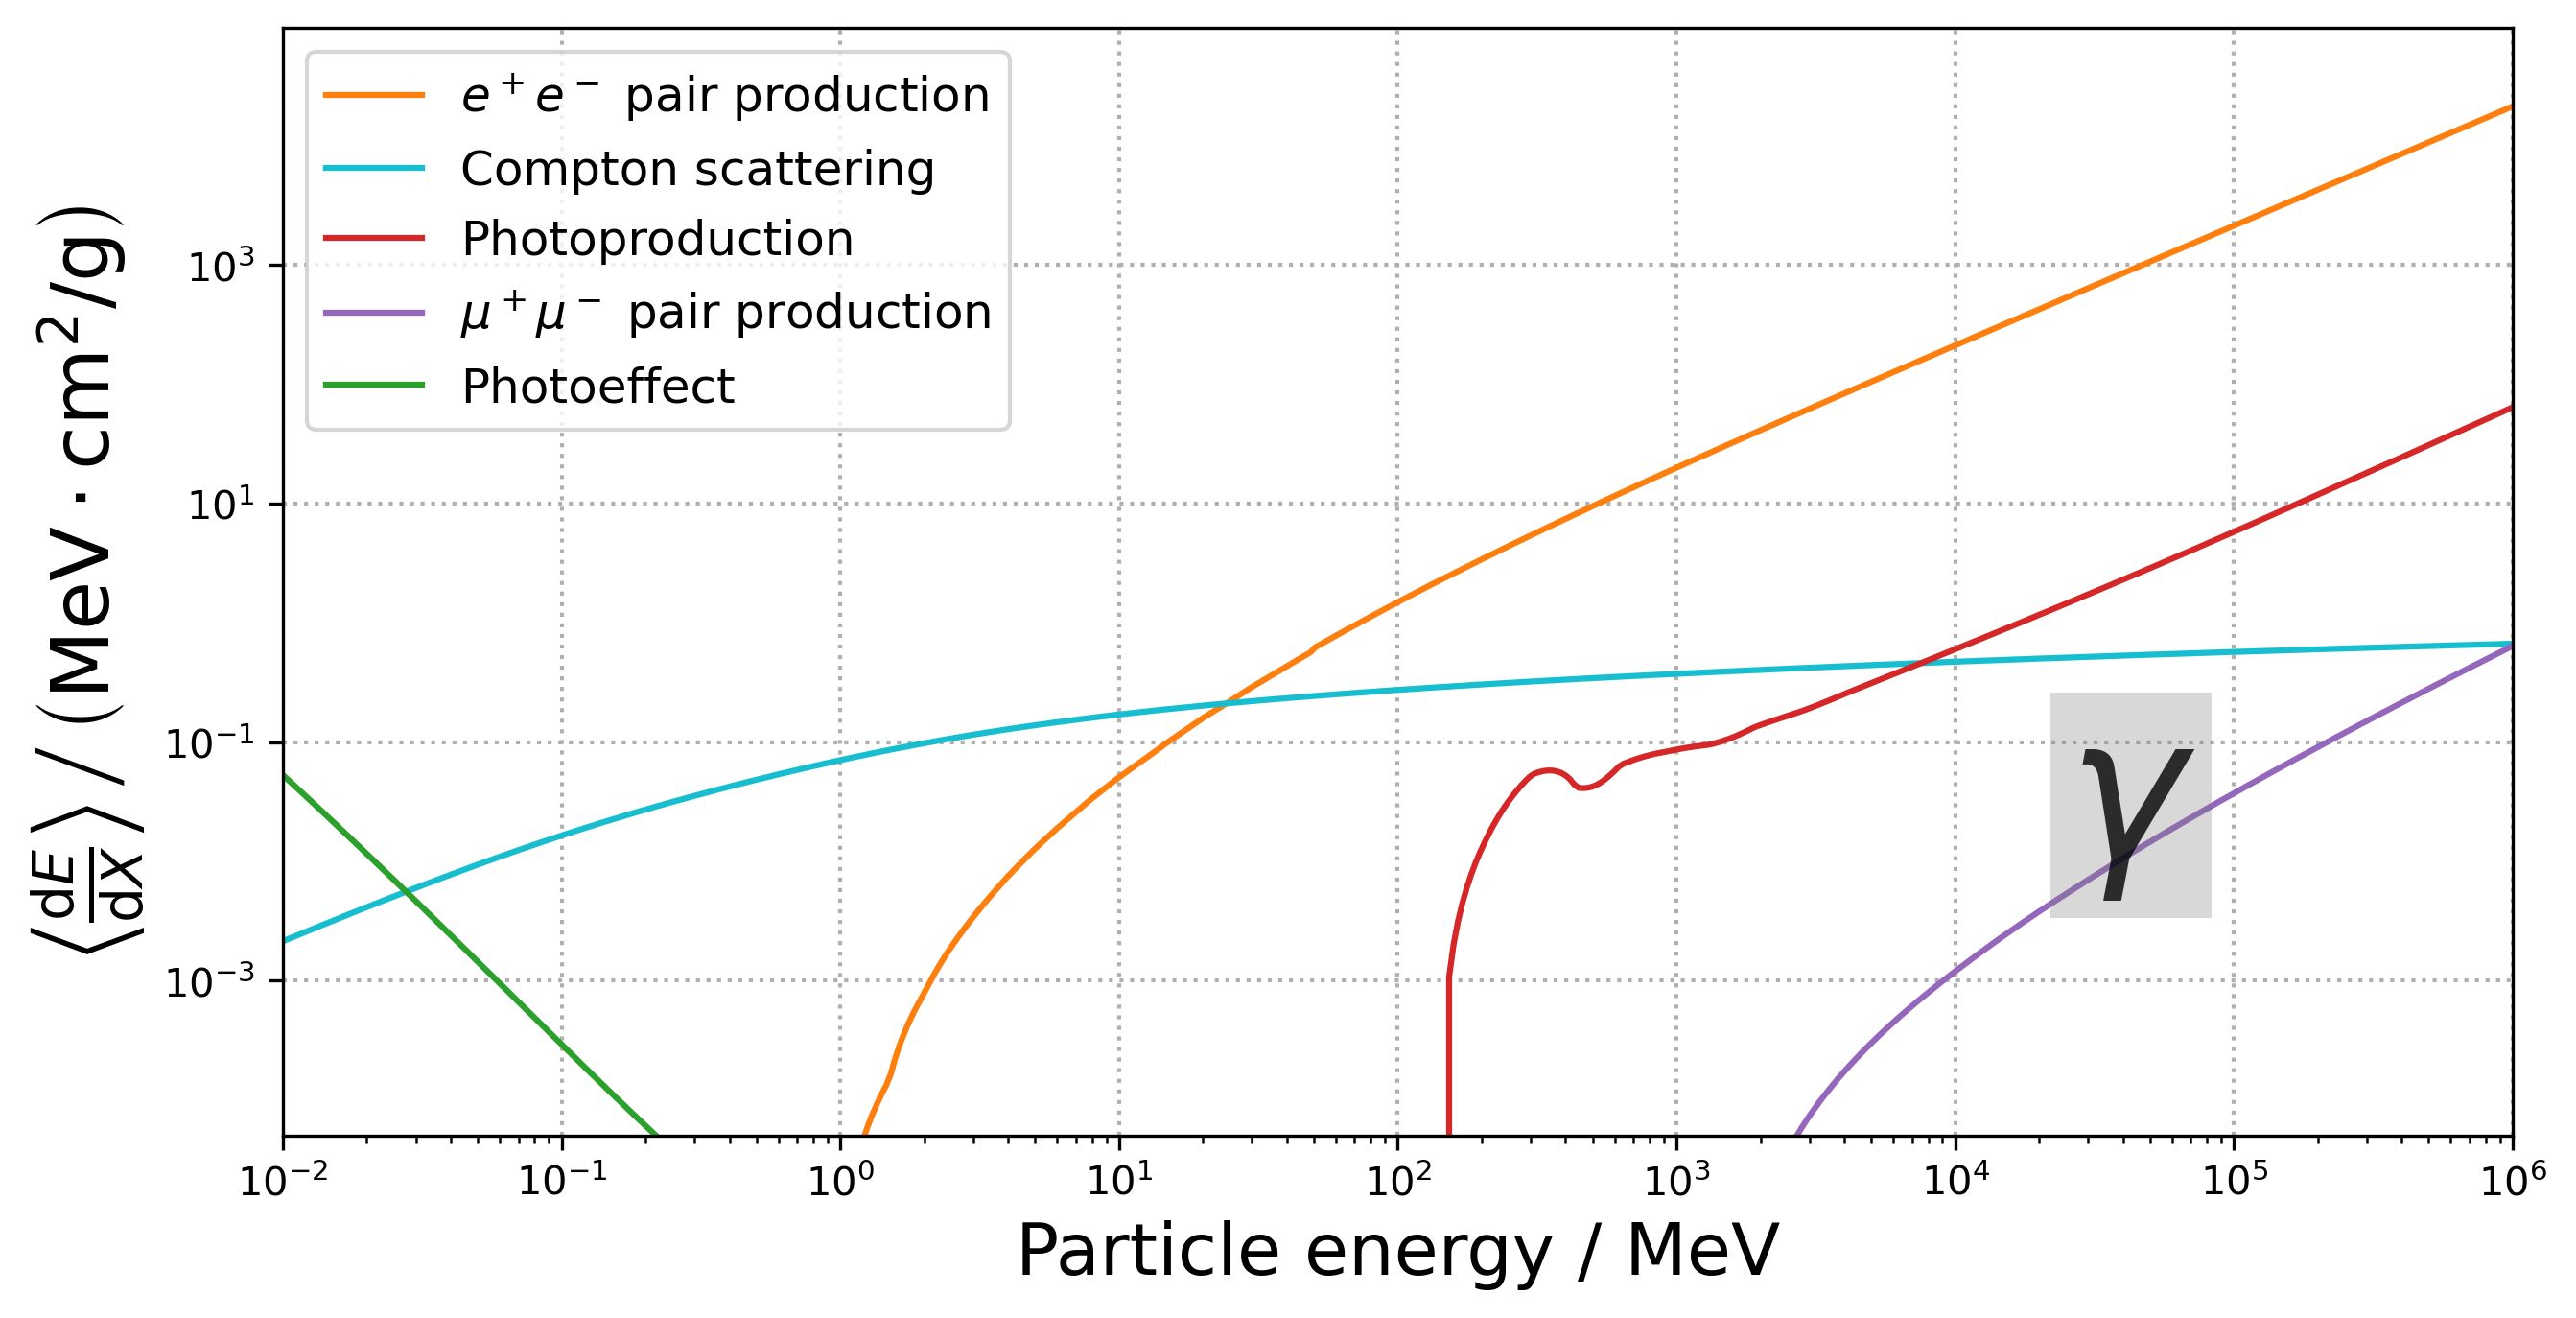
\includegraphics[width=0.9\textwidth]{plots/photon_dEdx.png}
    \end{figure}
    \vspace{-3mm}
    \begin{figure}
        \centering
        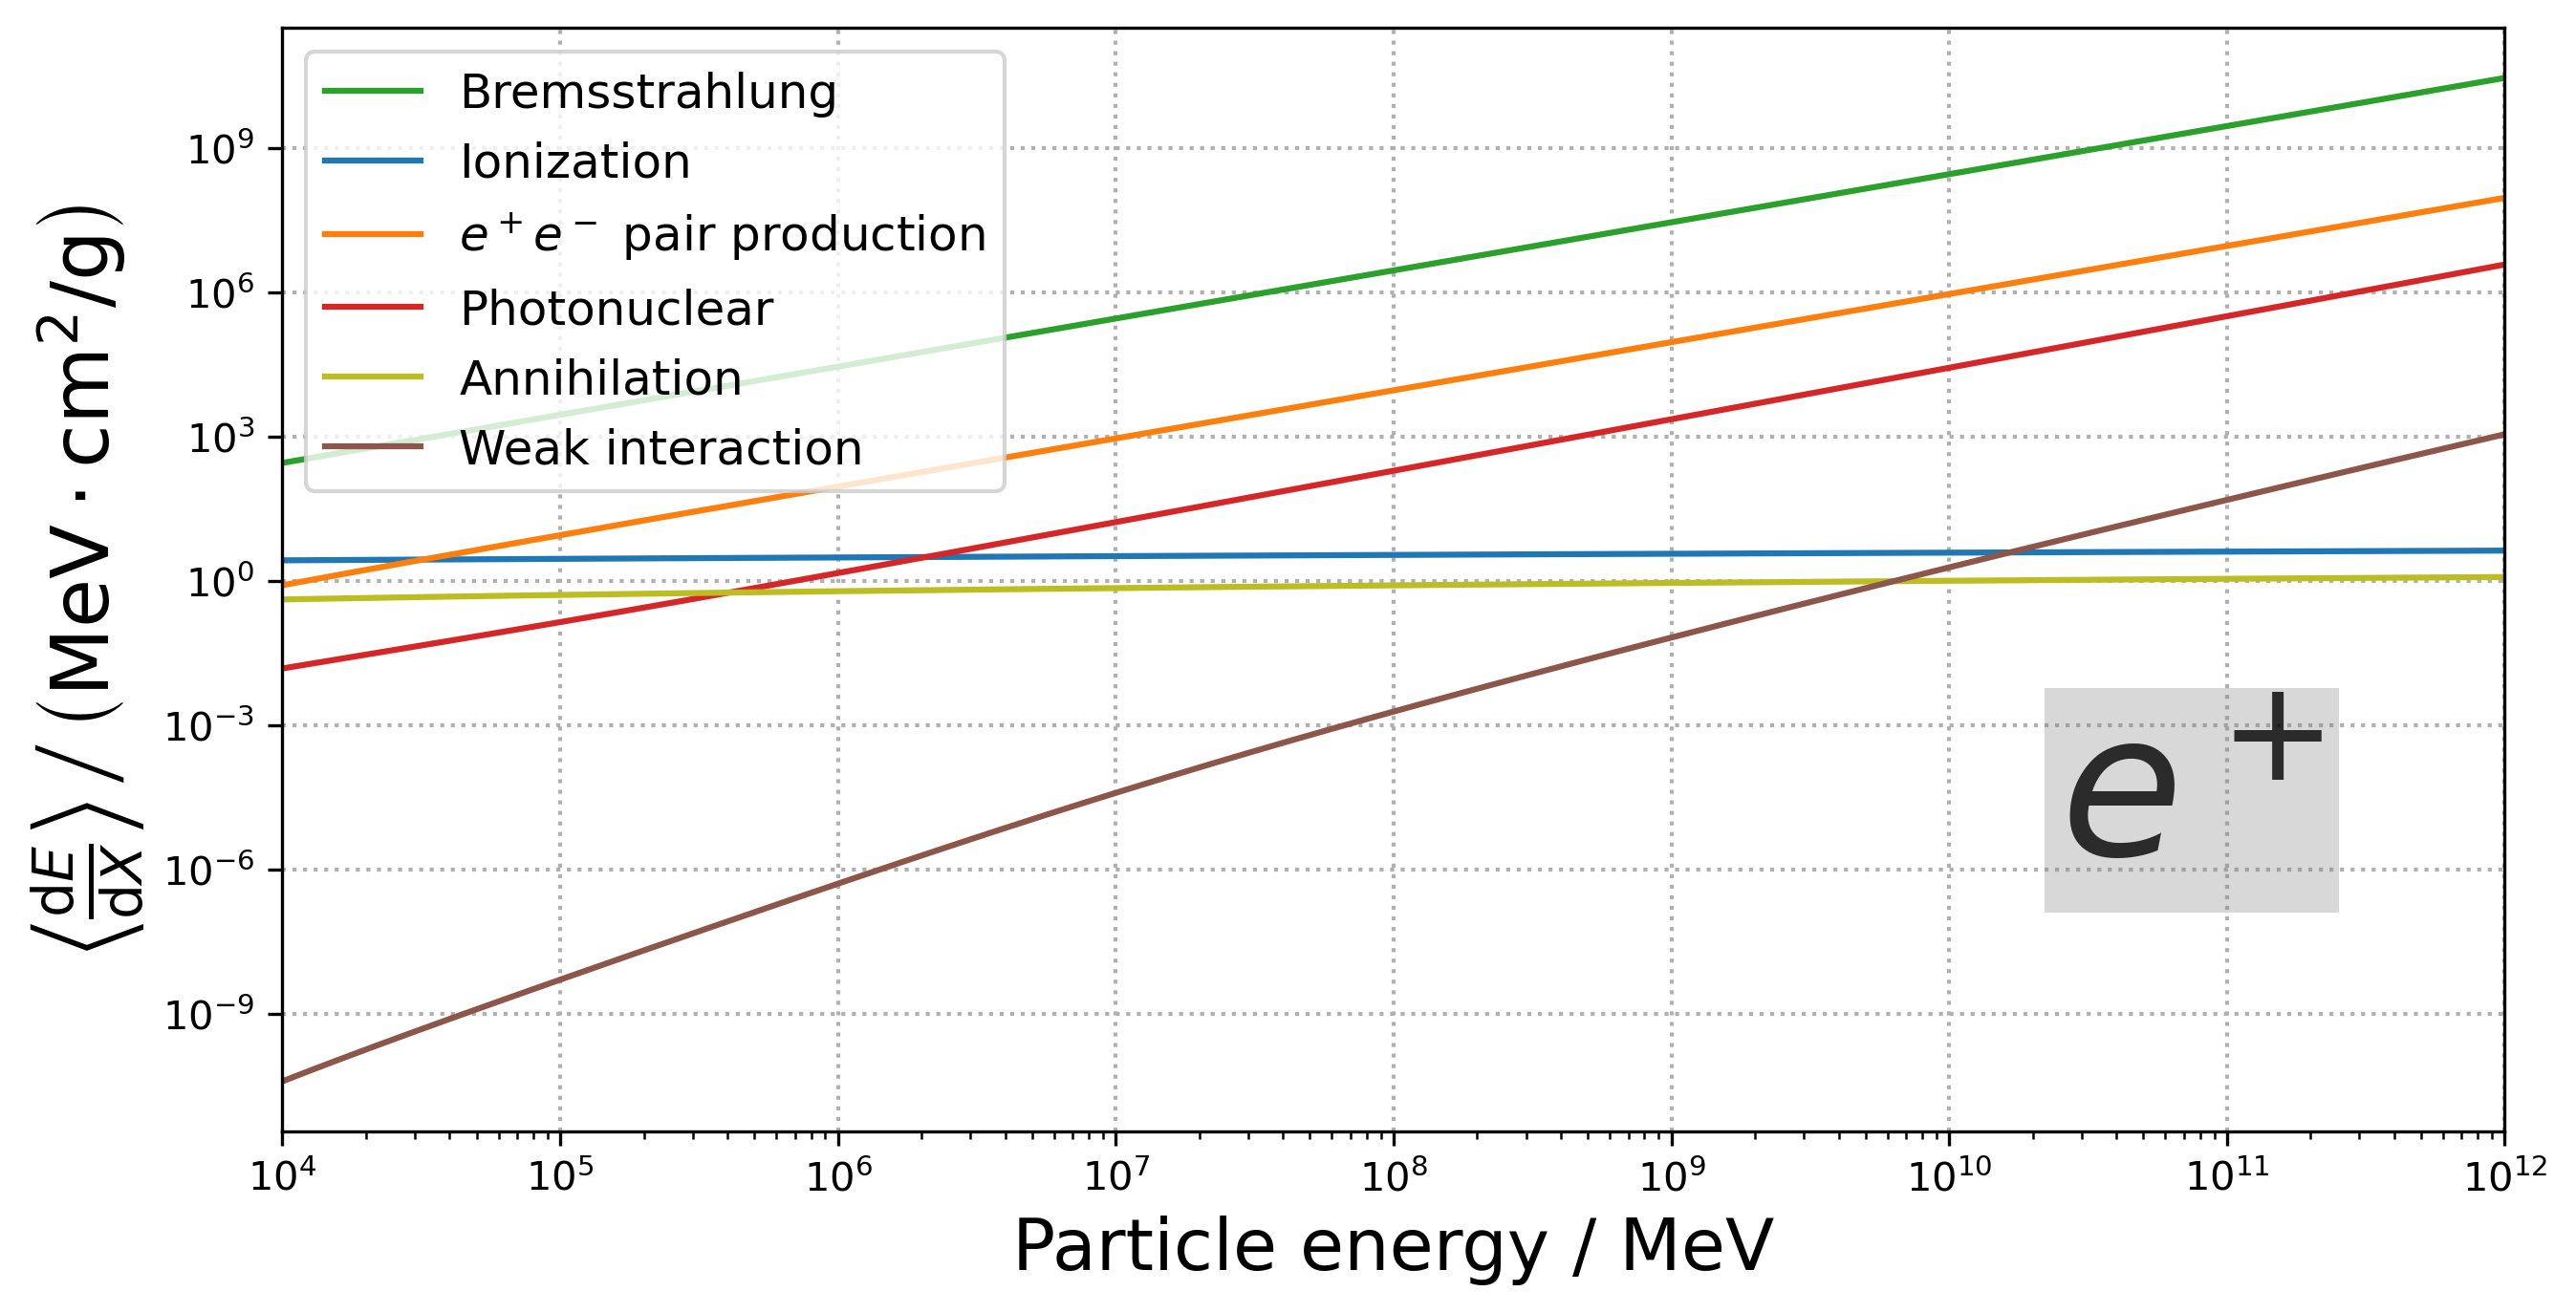
\includegraphics[width=0.9\textwidth]{plots/positron_dEdx.png}
    \end{figure}

    \end{column}
\end{columns}

\end{frame}



\begin{frame}[c]
    \begin{columns}[onlytextwidth]
    \begin{column}{0.45\textwidth}
        \textbf{Analysis of muon deflections}
        \begin{itemize}
            \item The main source of muon deflections is multiple scattering (scattering in continuous losses)
            \item However, deflection can also occur in individual, highly-stochastic interactions
            \begin{itemize}
                \item[$\rightarrow$] Both effects are implemented in PROPOSAL
            \end{itemize}
            \item We performed comparisons of muon deflections in PROPOSAL with other Monte Carlo tools (\textsc{Geant4}, MUSIC) and data
            \begin{itemize}
                \item[$\rightarrow$] We found them to be in good agreement
            \end{itemize}
        \end{itemize}

    \end{column}
        \begin{column}{0.55\textwidth}

            \begin{figure}
              %\vspace{-9pt}
              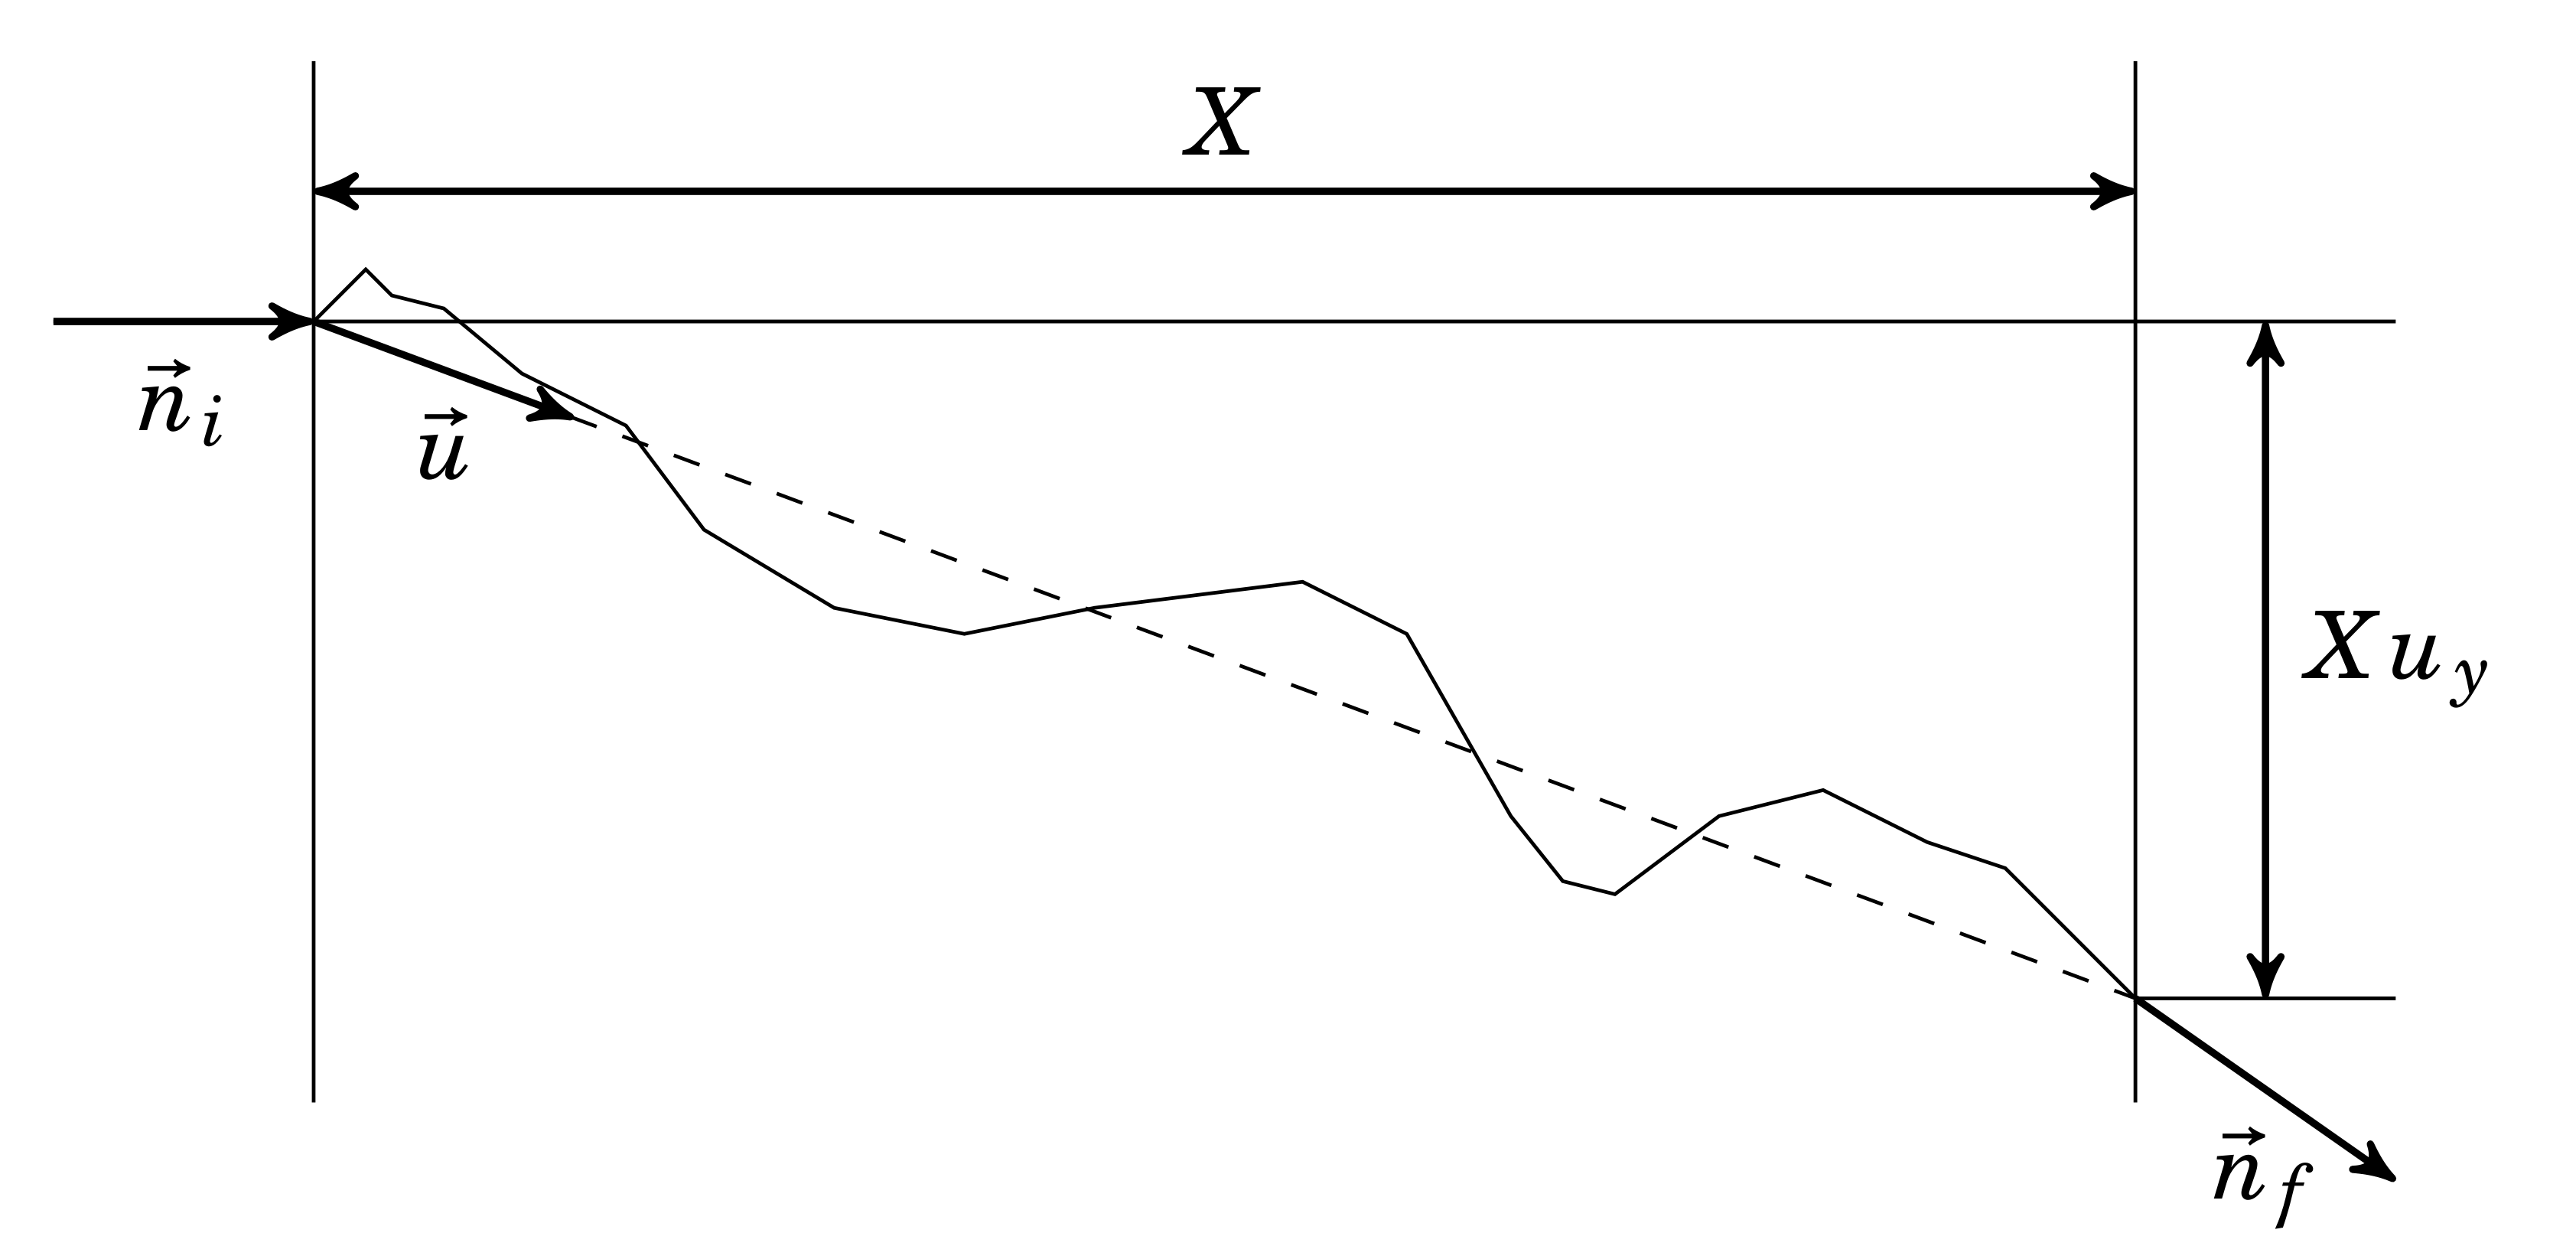
\includegraphics[width=0.8\linewidth, keepaspectratio]{plots/multiple_scattering_dunsch.png}
              \captionsetup{justification=centering}
              %\caption*{Paper by P.~Gutjahr et al., submitted to EPJ C \\(available as \href{https://arxiv.org/abs/2208.11902}{arXiv:2208.11902})}
            \end{figure}
        \vspace{3pt}
        \begin{figure}



            \begin{tikzpicture}[scale=0.7, every node/.style={scale=0.7}]
                \centering

                \coordinate (start) at (-1,0);
                \coordinate (kink) at (1.8, 0);
                \coordinate (end) at (4.5, 0.8);
                \coordinate (continue) at (4.5, 0);



                \draw [black, line width=0.6mm] (start) -- node[above] {$\mu$}  (kink);
                \draw [->, black, line width=0.6mm] (kink) -- node[above] {$\mu^\prime$}  (end);
                \draw [black, dashed, line width=0.2mm] (kink) -- (continue);

                \fill [red] (kink) circle (0.15) node[label=below: $\substack{\text{stochastic} \\ \text{interaction}}$]{};

                \pic [draw, "$\theta$", angle eccentricity=0.7, angle radius=2cm] {angle = continue--kink--end};

            \end{tikzpicture}
        \end{figure}  

        \end{column}
    \end{columns}
\end{frame}




\begin{frame}[c]
    \begin{columns}[onlytextwidth]
    \begin{column}{0.45\textwidth}
        \textbf{Analysis of muon deflections}
        \begin{itemize}
            \item We have investigated the influence of muon deflections on directional resolutions based on PROPOSAL simulations
            \item We performed simulations of muons with identical initial energies, and plotted the accumulated muon deflections for different final energies
            \begin{itemize}
                \item[$\rightarrow$] Accumulated deflection primarily depends on the final muon energy (independent of initial energy)
                \item[$\rightarrow$] We can see a potential impact of muon deflections on the angular resolution of KM3NeT at energies $E_\text{f} \leq \SI{1}{\tera\electronvolt}$
            \end{itemize} 
        \end{itemize}

    \end{column}
        \begin{column}{0.55\textwidth}
    		\begin{figure}
    		  %\vspace{-9pt}
    		  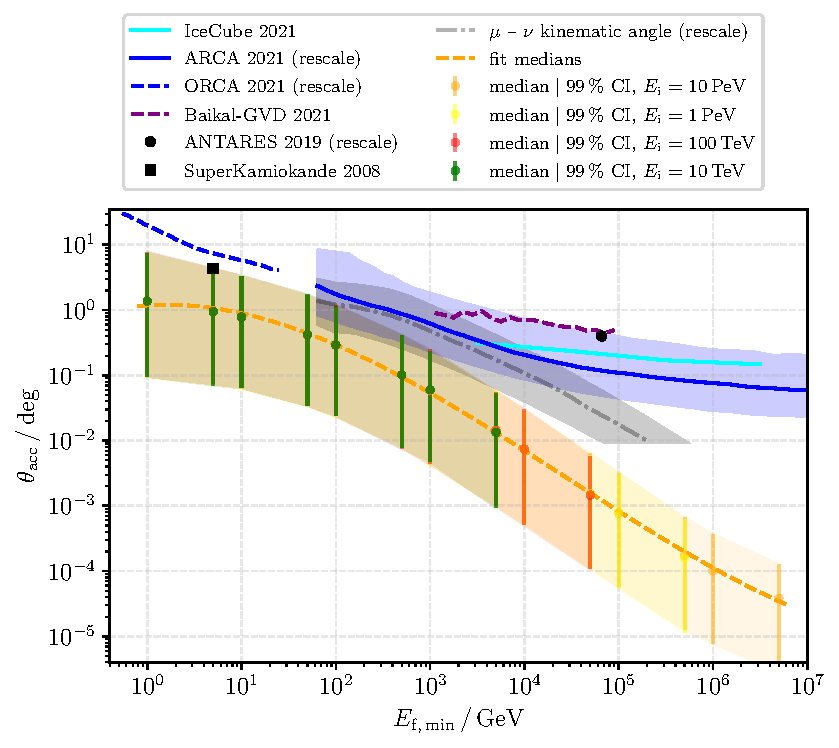
\includegraphics[width=\linewidth, height=.85\textheight, keepaspectratio]{plots/fit_median_defl_cut_10percent_only_poly_new_resolution_rescale_no_icecube_paper_final_all.pdf}
    		  \captionsetup{justification=centering}
    		  \caption*{Paper by P.~Gutjahr et al., accepted by EPJ C \\(available as \href{https://arxiv.org/abs/2208.11902}{arXiv:2208.11902})}
    		\end{figure}

        \end{column}
    \end{columns}
\end{frame}


\section{Applications}

\begin{frame}[plain,c,noframenumbering]
  \begin{center}
    \Huge Applications of PROPOSAL
  \end{center}
\end{frame}

\begin{frame}[c]
    \begin{columns}[onlytextwidth]
    \begin{column}{0.55\textwidth}
    \textbf{Neutrino observatories}
        \begin{itemize}
            \item Usage in the \textbf{IceCube} simulation chain
            \begin{itemize}
                \item[$\rightarrow$] PROPOSAL provides the energy losses of muons and taus along the particle track
                \item[$\rightarrow$] Estimation of background contamination, e.g. due to undetected muons in veto regions
            \end{itemize}
            \item Usage in \textbf{NuRadioMC}, a framework for radio neutrino simulations
            \begin{itemize}
                \item[$\rightarrow$] Estimation of radio contribution due to muon and tau energy losses in ice
            \end{itemize}
        \end{itemize}
    \end{column}
        \begin{column}{0.45\textwidth}
            \begin{figure}
                \centering
                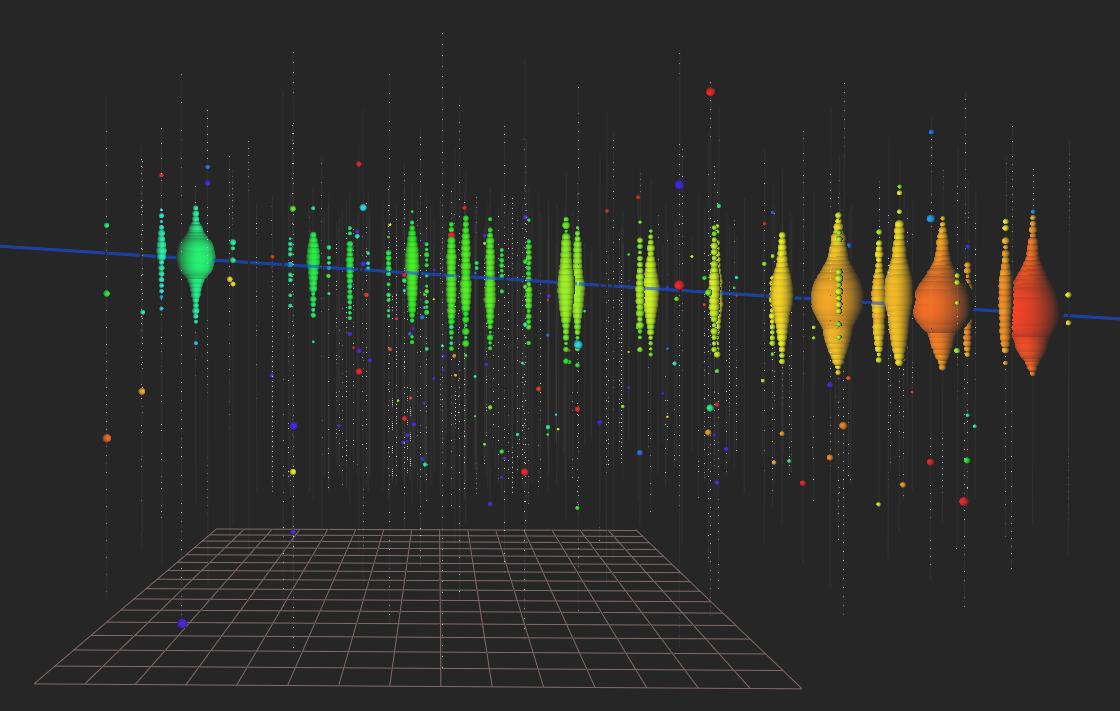
\includegraphics[width=0.9\textwidth]{images/Track.png}
                \credit{IceCube Collaboration}
            \end{figure}
        \end{column}
    \end{columns}
\end{frame}


\begin{frame}[c]
    \begin{columns}[onlytextwidth]
    \begin{column}{0.6\textwidth}
    \textbf{CORSIKA 8}
        \begin{itemize}
            \item CORSIKA~8: Newest version of the air shower simulation framework CORSIKA (currently under development)
            \begin{itemize}
                \item[$\rightarrow$] see: \url{gitlab.iap.kit.edu/AirShowerPhysics/corsika}
            \end{itemize}
            \item PROPOSAL is used in CORSIKA~8 as an electromagnetic and muonic shower model
            \begin{itemize}
                \item[$\rightarrow$] CORSIKA uses propagation steps provided by PROPOSAL modules
            \end{itemize}
        \end{itemize}

    \end{column}
        \begin{column}{0.4\textwidth}
            \begin{figure}
                \centering
                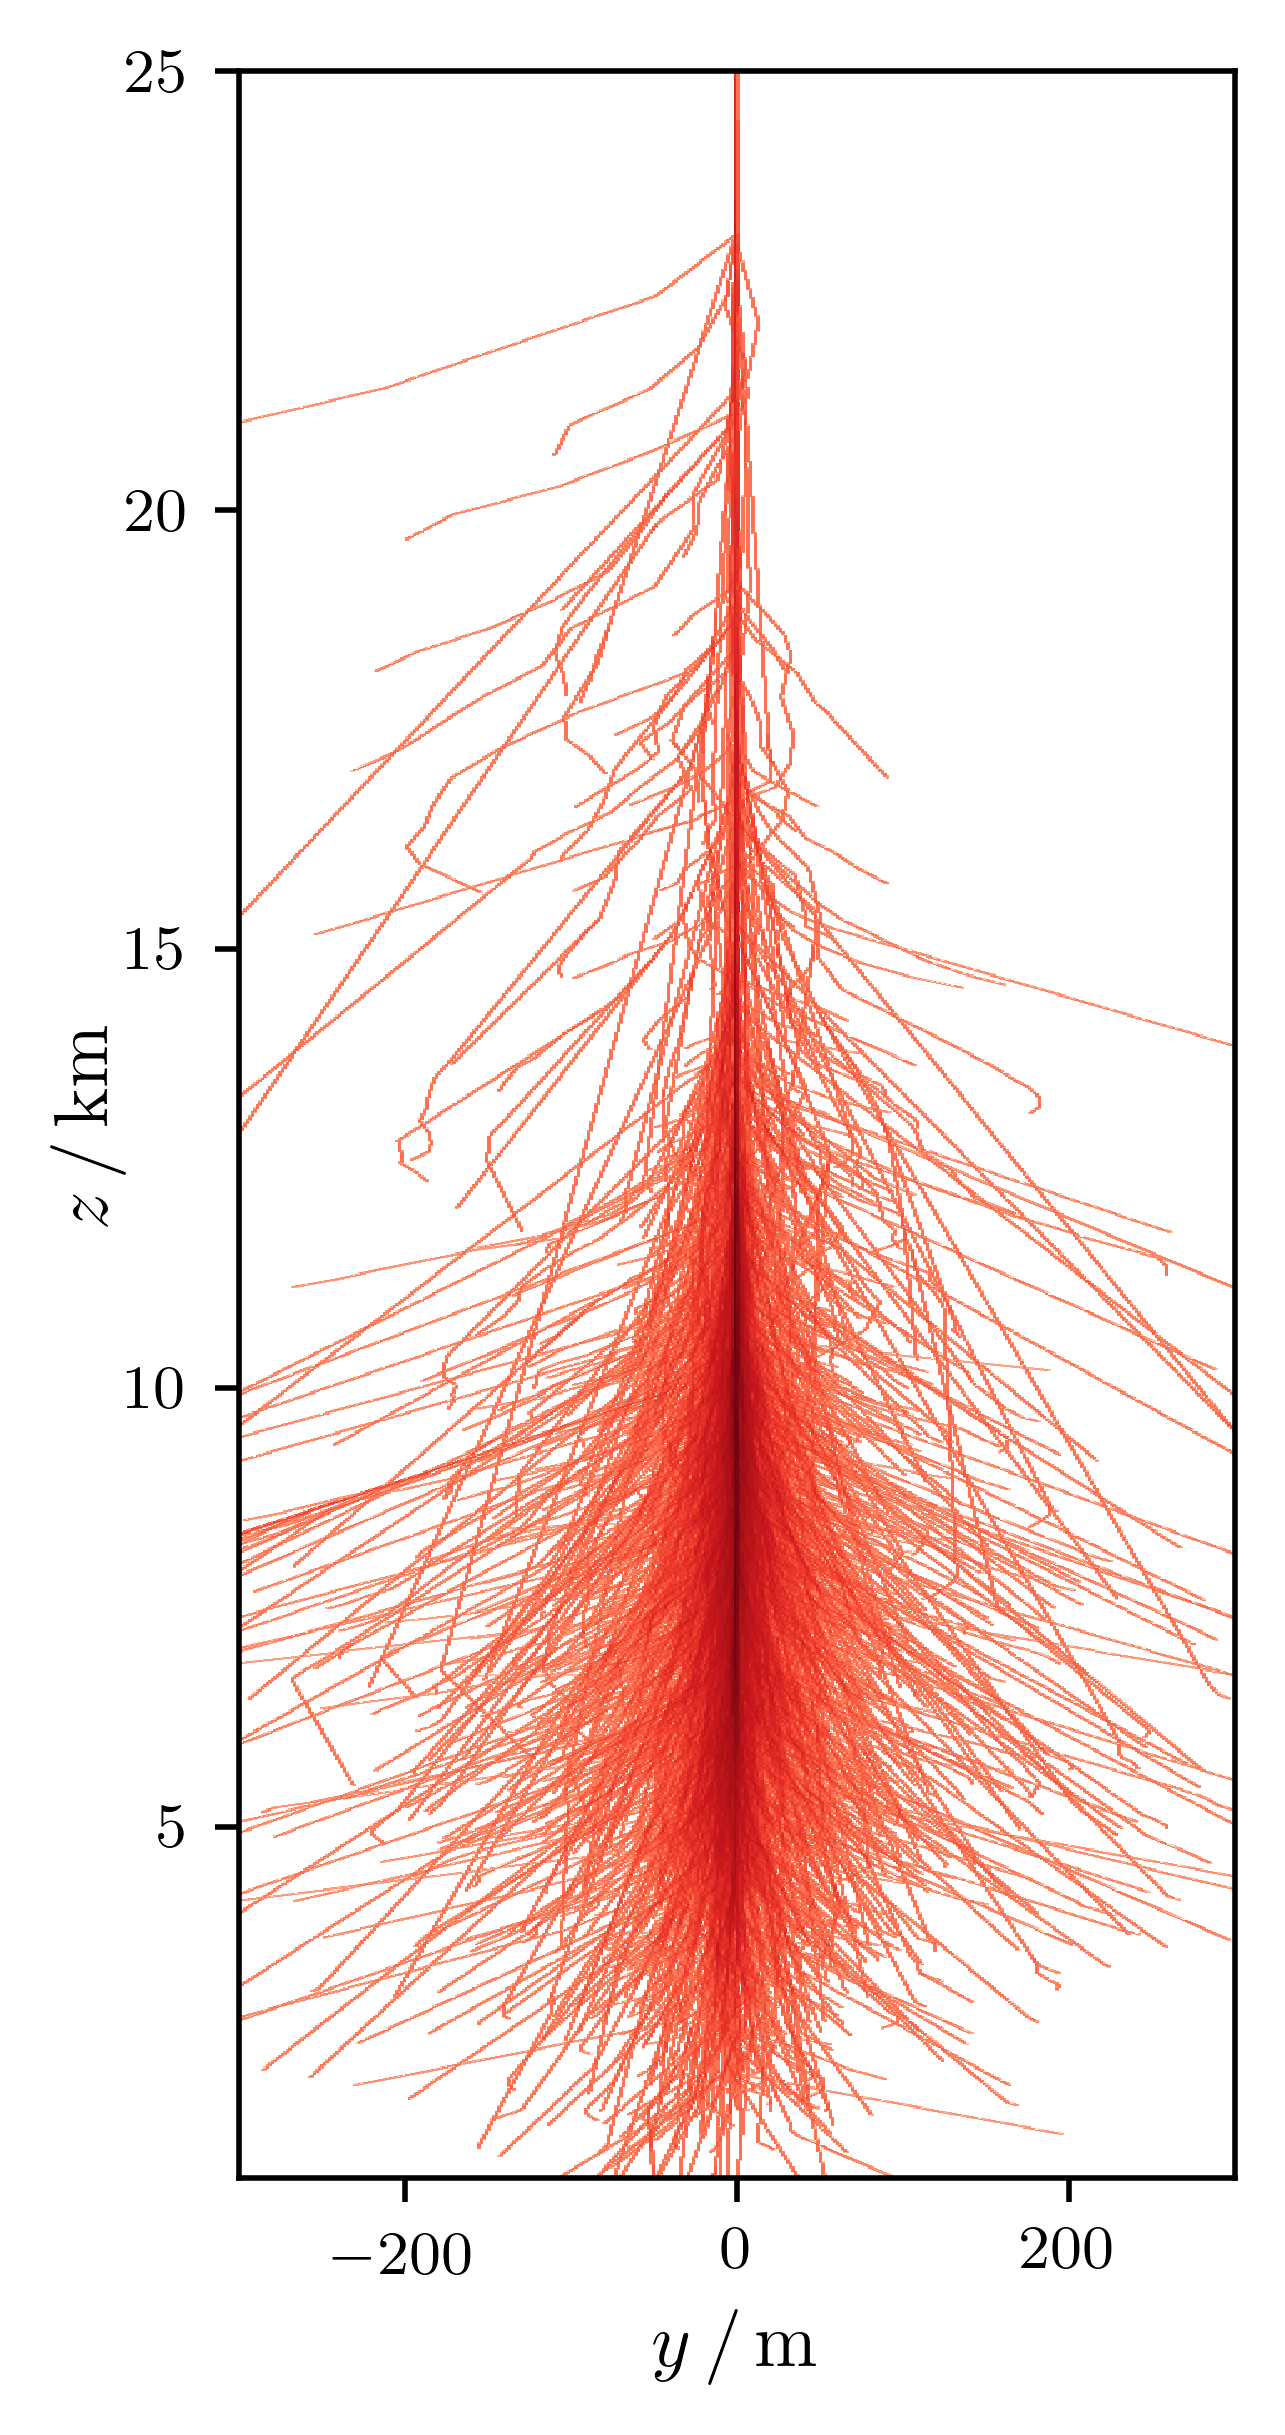
\includegraphics[width=0.6\textwidth]{plots/shower.png}
                \caption*{\SI{1}{\tera\electronvolt} $e^-$ shower simulated with CORSIKA 8}
            \end{figure}
        \end{column}
    \end{columns}
\end{frame}


\begin{frame}[c]
    \begin{figure}
        \centering
        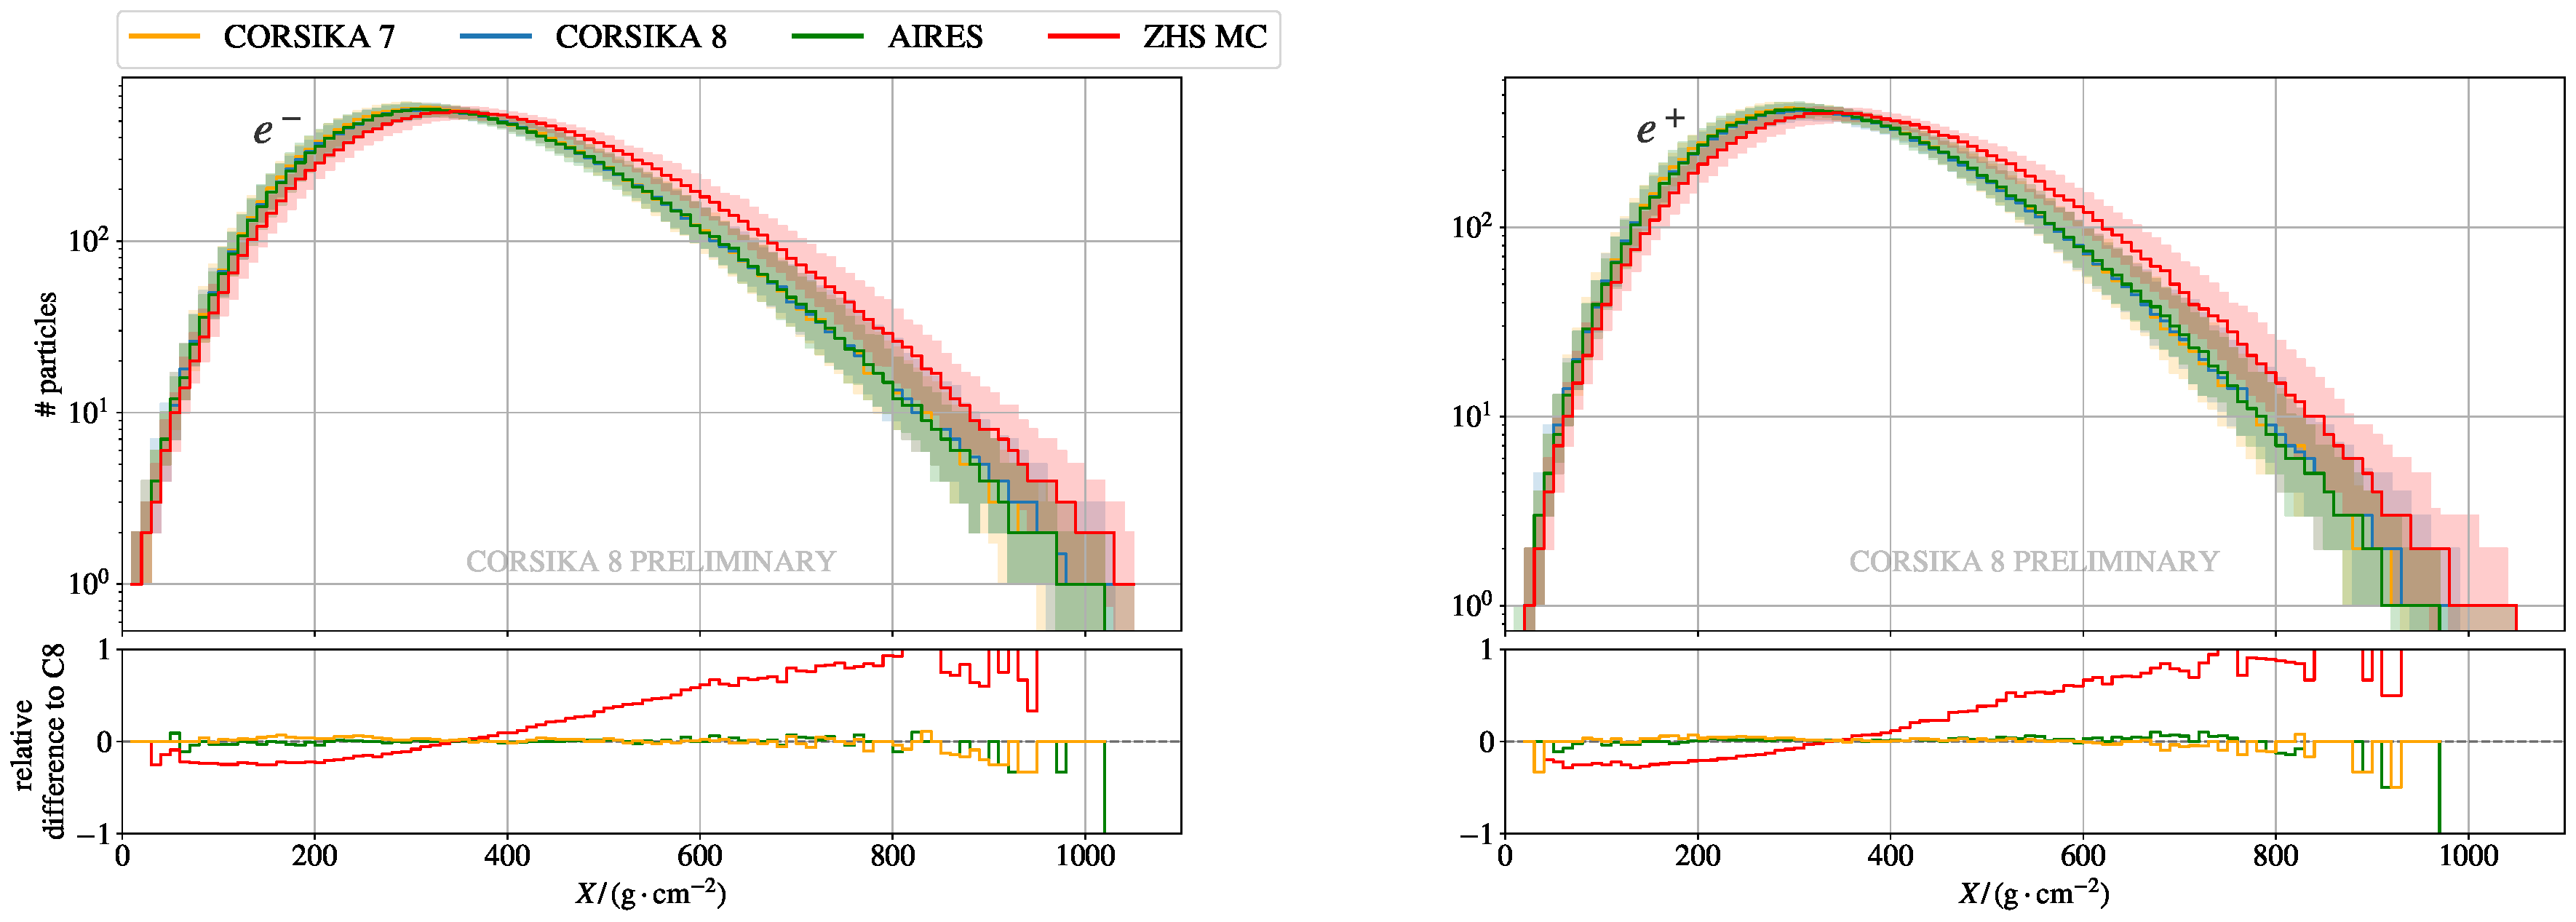
\includegraphics[width=0.85\textwidth]{plots/longitudinal_profile.pdf}
        \caption*{Longitudinal profile for 200 electromagnetic showers, initiated by \SI{1}{\tera\electronvolt} $e^-$}
    \end{figure}
    \begin{itemize}
        \item First comparisons of CORSIKA~8 results with other simulation frameworks are promising
    \end{itemize}

    \hspace{20pt} $\Rightarrow$ See \href{https://pos.sissa.it/395/428/}{PoS(ICRC2021)428}

\end{frame}



\begin{frame}[c]
    \begin{columns}[onlytextwidth]

    \begin{column}{0.5\textwidth}
        \textbf{Muography:}
        \begin{itemize}
            \item Non-invasive imaging technique using Cosmic Ray muons
            \begin{itemize}
                \item[$\rightarrow$] Trace muon number to observe density anomalies
            \end{itemize}
            \item PROPOSAL is a well-suited tool to provide the necessary muon simulations
            \begin{itemize}
                \item[$\rightarrow$] Currently analyzing the possibilities to use muography in mining with PROPOSAL simulations
            \end{itemize}
        \end{itemize}
    \end{column}

    \begin{column}{0.5\textwidth}
        \begin{figure}
            \begin{tikzpicture}[scale=0.85, every node/.style={scale=0.85}]
                \centering

                \coordinate (A) at (0, 0);

                % ground
                \draw[draw=none, fill=gray, fill opacity=1.0] ($ (A) + (-3.5,-2.5) $) rectangle ++(7, 5);

                % sky
                \draw[draw=none, fill={rgb:red,0.33;green,0.5;blue,0.98}, fill opacity=0.5] ($ (A) + (-3.5,2.5) $) rectangle ++(7, 1);
                \node[draw=none] at ($ (A) + (0.0, 3) $) {Sky};

                % mining shaft
                \draw[draw=none, fill={rgb:black,1;white,2}, fill opacity=1.0] ($ (A) + (2, -1.5) $) rectangle ++(0.25, 4.0);
                \draw[draw=none, fill={rgb:black,1;white,2}, fill opacity=1.0] ($ (A) + (-2.0, -1.5) $) rectangle ++(4, 0.5);

                \node[draw=none] at ($ (A) + (0.8, -1.25) $) {Mining shaft};

                % detector
                \node [cylinder, shape border rotate=90, draw,minimum height=0.40cm,minimum width=0.25cm, aspect=0.4] (detector) at ($ (A) + (-0.5, -1.3) $) {};

                % impurity
                \draw[draw=none,fill=black, fill opacity=0.7] ($ (A) + (0, 0.07) $) ellipse (0.3cm and 0.1cm);
                \node[draw=none, text width=1cm] at ($ (A) + (0.9, 0.07) $) {Anomaly};

                % muons
                \draw [densely dotted, blue, line width=0.25mm] ($ (A) + (-2.5, 3.0) $) -- ($ (detector) + (0.2, -0.5) $) node [near start, above, xshift=1ex] (TextNode) {$\mu$};

                \draw [densely dotted, blue, line width=0.25mm] ($ (A) + (-1.0, 3.0) $) -- ($ (detector) + (0.1, -0.5) $) node [near start, above, xshift=1ex] (TextNode) {$\mu$};

                \draw [densely dotted, blue, line width=0.25mm] ($ (A) + (1.0, 3.0) $) -- ($ (A) + (0, 0.07) $) node [pos=0.4, above, xshift=-1ex] (TextNode) {$\mu$};

            \end{tikzpicture}
        \end{figure}  
    \end{column}

    \end{columns}
\end{frame}



\section{Summary and outlook}

\begin{frame}[plain,c,noframenumbering]
  \begin{center}
    \Huge Summary
  \end{center}
\end{frame}


\begin{frame}[c]
    \begin{columns}[onlytextwidth]
        \begin{column}{0.7\textwidth}
            \textbf{Summary}
            \begin{itemize}
                \item C\texttt{++}/Python framework to propagate high-energy leptons and photons 
                \begin{itemize}
                    \item[$\rightarrow$] Easy python installation: Try: \texttt{pip install proposal}
                \end{itemize}
                \item PROPOSAL can be used for different use cases
                \begin{itemize}
                    \item[$\rightarrow$] I have shown a few, but there are many other applications
                \end{itemize}
                \item Study: Muon scattering might have an influence on directional reconstructions in KM3Net
                %\item PROPOSAL is used in a wide field of applications (e.g. IceCube, CORSIKA~8)
                \item Actively maintained and developed as an open-source project
                %\begin{itemize}
                %    \item[\rightarrow] Visit us on GitHub: \url{github.com/tudo-astroparticlephysics/PROPOSAL}
                %\end{itemize}
            \end{itemize}


              \begin{center}
                \colorbox{light-gray}{
            \begin{minipage}[ht]{0.75\linewidth}
              \begin{center}
              \textbf{Find the PROPOSAL repository under:}\\ \url{github.com/tudo-astroparticlephysics/PROPOSAL} %\vspace{0.5em}\\
              \end{center}
            \end{minipage}
            \begin{minipage}[ht]{0.24\linewidth}
              \centering
                
\includegraphics[width=0.66\linewidth, valign=t]{plots/qr_proposal_transparent.png}
            \end{minipage}
                }
              \end{center}
            
        \end{column}
        \begin{column}{0.3\textwidth}
            \begin{center}
                \begin{tikzpicture}[scale=1, transform shape]
                    \newlength{\photodim}
                    \setlength{\photodim}{0.8cm}%
                    \newlength{\borderdim}
                    \setlength{\borderdim}{0.3mm}%

                    \node[circle, draw=tugreen, line width=\borderdim, inner
                    sep=\photodim, fill overzoom image=images/collaboration.png] at (1.8,0) {};

                    \node[circle, draw=tugreen, fill=white, line width=\borderdim, inner
                    sep=\photodim, fill overzoom image*={angle=30,clip,trim=0.0cm 0.0cm 0.0cm 0.0cm}{plots/shower_raw.png}] at (0,1) {};

                    \node[circle, draw=tugreen, line width=\borderdim, inner
                    sep=\photodim, fill overzoom image*={clip,trim=0 3cm 0 0}{images/Track.png}] at (1.8,2) {};


                    \node[circle, draw=tugreen, line width=\borderdim, inner
                    sep=\photodim, fill overzoom image*={clip,trim=2cm 2cm 2cm 1cm}{plots/tracks.png}] at (0,3) {};

                    \node[circle, draw=tugreen, line width=\borderdim, inner
                    sep=\photodim, fill overzoom image=logos/cpp-python.png] at (1.8,4) {};
                \end{tikzpicture}
            \end{center}

        \end{column}
    \end{columns}
\end{frame}


\end{document}
